% Compile here: latexmk -pdf report_en.tex
\documentclass[12pt,a4paper]{article}
\usepackage{cmap}
\usepackage[utf8]{inputenc}
\usepackage[T1]{fontenc}
\usepackage[english]{babel}
\usepackage{amsmath,amssymb,bm}
\usepackage{graphicx,float,booktabs,geometry,array,needspace}
\usepackage[justification=raggedright,singlelinecheck=false]{caption}
\usepackage[expansion=false]{microtype}
\usepackage{xcolor}
\usepackage{hyperref}
\geometry{margin=2.2cm}
\setlength{\emergencystretch}{2em}
\AddToHook{cmd/subsection/before}{\Needspace{8\baselineskip}}
\hypersetup{colorlinks=true,linkcolor=black,citecolor=black,urlcolor=blue,
 pdftitle={Reservoir, spin and polarization dynamics of a polariton condensate},pdfauthor={Korostelev Nikita}}
\graphicspath{{../results/figures/report3/}}
\makeatletter
\setlength{\@fptop}{0pt}
\setlength{\@fpsep}{12pt}
\setlength{\@fpbot}{0pt plus 1fil}
\makeatother
\usepackage{longtable}
\setlength{\LTpre}{8pt}
\setlength{\LTpost}{8pt}
\title{Reservoir, spin and polarization dynamics of a polariton condensate}
\author{Korostelev Nikita}
\date{}
\begin{document}
\maketitle
\clearpage



\section*{Aim of the study}

The previous report, \emph{Dynamics and spatial structure of exciton-polariton condensates under nonresonant pumping}, used a scalar condensate and one reservoir. Here we add an inactive reservoir, two circular components, constant coherent coupling, and momentum-dependent TE--TM splitting.

We examine reservoir transients, the response to pump polarization, and changes in phase dynamics and spatial polarization. Homogeneous calculations are followed by Gaussian-spot and annular pumping; Stokes parameters then provide a common description of the polarization states.

The condensation parameters are retained. Additional coefficients and their literature basis are given in Appendix A; they are not recalibrated using the earlier dispersion report.

\section{Active and inactive reservoirs}

\subsection{Extension of the scalar model}

In the previous model, the condensate field \(\psi\) and reservoir density \(n_R\) obeyed

\[
\begin{gathered}
i\hbar\partial_t\psi=
\left[-K\nabla^2+g_C|\psi|^2+g_R(n_R+\eta P_A)
+\frac{i\hbar}{2}(Rn_R-\gamma_C)\right]\psi,
\\
\partial_t n_R=P_A-(\gamma_R+R|\psi|^2)n_R,
\qquad K=\frac{\hbar^2}{2m}.
\end{gathered}
\tag{1}\label{eq:1}
\]

Here, \(P_A\) replaces the previous pump notation \(P\), distinguishing reservoir injection from the external pump introduced below.

The instantaneous energy shift \(g_R\eta P_A\) is replaced by a dynamical inactive reservoir \(n_I\). The external pump \(P_{\rm in}\) populates this reservoir, which supplies the active reservoir \(n_A\) at rate \(Wn_I\). Stimulated scattering from \(n_A\) feeds the condensate:

\[
\begin{aligned}
i\hbar\partial_t\psi&=\left[-K\nabla^2+g_C|\psi|^2+g_A n_A+g_I n_I
+\frac{i\hbar}{2}(Rn_A-\gamma_C)\right]\psi,\\
\partial_t n_A&=Wn_I-(\gamma_A+R|\psi|^2)n_A,\\
\partial_t n_I&=P_{\rm in}-(\gamma_I+W)n_I.
\end{aligned}
\tag{2}\label{eq:2}
\]

Both reservoirs shift the condensate energy; \(g_R\eta P_A\) is not added again. The model structures follow Refs. \cite{ref1,ref2}.

To match the models, we choose

\[
g_A=g_R,\qquad \gamma_A=\gamma_R,\qquad
P_{\rm in}=\frac{\gamma_I+W}{W}P_A,\qquad
\frac{g_I}{W}=g_R\eta.
\tag{3}\label{eq:3}
\]

Under constant pumping, \(n_I^*=P_A/W\). The particle supply and additional energy shift therefore reproduce their previous values:

\[
Wn_I^*=P_A,\qquad g_I n_I^*=g_R\eta P_A.
\]

The stationary solutions of the scalar model are thus preserved. In the homogeneous case, the condensation threshold is also unchanged:

\[
P_{\rm th}=\frac{\gamma_C\gamma_A}{R}
=0.43333\;\mu\mathrm m^{-2}\mathrm{ps}^{-1}.
\]

This matching does not require the transient dynamics to coincide.

\subsection{Response to pump turn-on and turn-off}

Define the particle transfer rate into the active reservoir as \(Q_A=Wn_I\). Equations (2) and (3) give

\[
\tau_I\frac{dQ_A}{dt}=P_A-Q_A,
\qquad \tau_I=\frac{1}{\gamma_I+W}.
\tag{4}\label{eq:4}
\]

The supply to the active reservoir now responds on a finite time scale. For the main parameter set, \(\tau_I=9.63\) ps.

The comparison uses \(P_A=1.5P_{\rm th}\), initially empty reservoirs, and the same weak condensate seed. Both models approach

\[
n_C^*=\frac{P_A-P_{\rm th}}{\gamma_C}
=1.19048\;\mu\mathrm m^{-2}.
\]

Condensate growth starts later in the model with two reservoirs. Half of the steady-state density is first reached at 159.1 ps in the previous model and at 188.0 ps in the extended model. This delay reflects the entire transient and is not equal to \(\tau_I\).

After turn-off, the inactive reservoir continues to feed the active reservoir and slows the condensate decay (Fig.~\ref{fig:1}). The single-reservoir model also retains particles in its active reservoir, but its external supply stops immediately.


\begin{figure}[H]
\centering
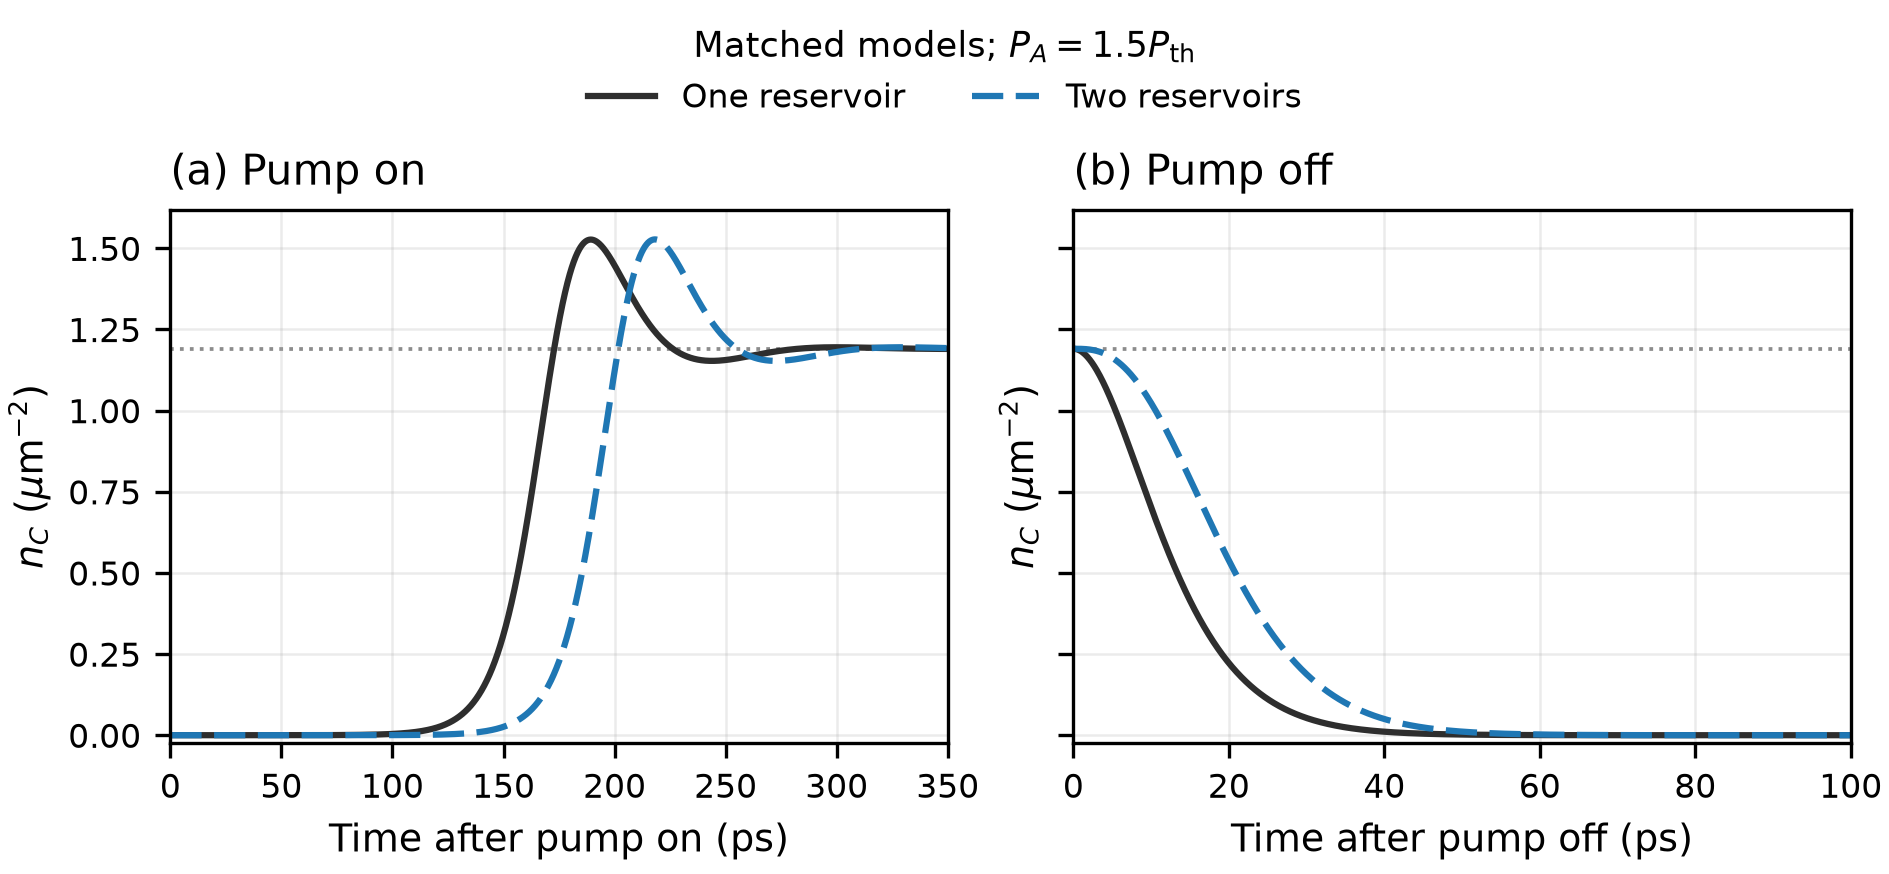
\includegraphics[width=0.96\textwidth]{../results/figures/report3/P1_reservoir_switching.png}
\caption{Condensate density after pump turn-on (a) and turn-off (b) for the single-reservoir and matched two-reservoir models. The on-state pump is \(P_A=1.5P_{\rm th}\); both runs use the same seed and initially empty reservoirs. The dotted line marks the common steady density. Time is measured from each switching event; turn-off occurs at 1000 ps.}
\label{fig:1}
\end{figure}

\section{Two spin components of the condensate}

\subsection{Model equations}

The circular fields \(\psi_\pm\) describe the two optically active angular-momentum projections along the cavity growth axis, not orbital circulation in the cavity plane. Their densities are \(n_\pm=|\psi_\pm|^2\); each has an active and an inactive reservoir.

Before adding TE--TM splitting, we use

\[
\begin{aligned}
i\hbar\partial_t\psi_\sigma
&=\left[-K\nabla^2+V_\sigma
+\frac{i\hbar}{2}(Rn_{A,\sigma}-\gamma_C)\right]\psi_\sigma
-J\psi_{-\sigma},\\
V_\sigma&=\alpha_1n_\sigma+\alpha_2n_{-\sigma}
+g_A n_{A,\sigma}+g_I n_{I,\sigma},\\
\partial_t n_{A,\sigma}
&=Wn_{I,\sigma}-(\gamma_A+Rn_\sigma)n_{A,\sigma}
+\Gamma_{s,A}(n_{A,-\sigma}-n_{A,\sigma}),\\
\partial_t n_{I,\sigma}
&=P_{{\rm in},\sigma}-(\gamma_I+W)n_{I,\sigma}
+\Gamma_{s,I}(n_{I,-\sigma}-n_{I,\sigma}),
\qquad \sigma=\pm.
\end{aligned}
\tag{5}\label{eq:5}
\]

The coefficients \(\alpha_1\) and \(\alpha_2\) give interaction energy shifts for equal and opposite circular polarizations. Reservoir spin relaxation, proportional to \(\Gamma_s\), transfers particles between reservoir components while conserving their sum \cite{ref3}. Cross-spin reservoir interaction coefficients are zero.

Here \(J=0\). The diagonal term \(\alpha_2n_{-\sigma}\) changes phase evolution without directly transferring condensate particles; coherent transfer through \(J\) is considered in Chapter 3.

All density-dependent terms are local. Distinct spatial points are coupled by \(-K\nabla^2\); reservoir diffusion and nonlocal density integrals are absent.

\subsection{Density dependence on pump polarization}

For the homogeneous problem, we set

\[
P_{A,\pm}=sP_{\rm th}(1\pm\epsilon),\qquad
P_{{\rm in},\pm}=\frac{\gamma_I+W}{W}P_{A,\pm}.
\tag{6}\label{eq:6}
\]

The rescaled pump parameters \(P_{A,\pm}\) differ from the actual transfers \(Q_{A,\pm}=Wn_{I,\pm}\) when the inactive reservoir undergoes spin relaxation. Varying \(\epsilon\) preserves the total pump \(2sP_{\rm th}\); we use \(s=2\).

For \(J=0\), if both components have nonzero steady-state densities, gain-loss balance gives \(n_{A,+}^*=n_{A,-}^*=\gamma_C/R\). Writing

\[
D_I=\frac{\gamma_I+W}{\gamma_I+W+2\Gamma_{s,I}},
\]

we obtain

\[
n_{I,\pm}^*=\frac{sP_{\rm th}}{W}(1\pm\epsilon D_I),
\qquad
n_\pm^*=\frac{\gamma_A}{R}\left[s(1\pm\epsilon D_I)-1\right].
\tag{7}\label{eq:7}
\]

These expressions apply when both predicted densities are positive, that is, \(s(1-|\epsilon|D_I)>1\). For the chosen parameters, \(D_I=0.34180\), and this condition holds throughout \(-1\le\epsilon\le1\).

The normalized condensate imbalance, or degree of circular polarization, is

\[
z=\frac{n_+-n_-}{n_++n_-}=\frac{s\epsilon D_I}{s-1}.
\tag{8}\label{eq:8}
\]

For \(s=2\), \(z=0.68360\epsilon\). Inactive-reservoir spin relaxation reduces the supply imbalance. Equal active-reservoir densities can therefore support unequal condensate densities. Integration reproduces Eq. (7) (Fig.~\ref{fig:2}): at \(\epsilon=0.3\), \(n_+^*=2.86924\), \(n_-^*=1.89267\;\mu\mathrm m^{-2}\), and \(z=0.20508\).


\begin{figure}[H]
\centering
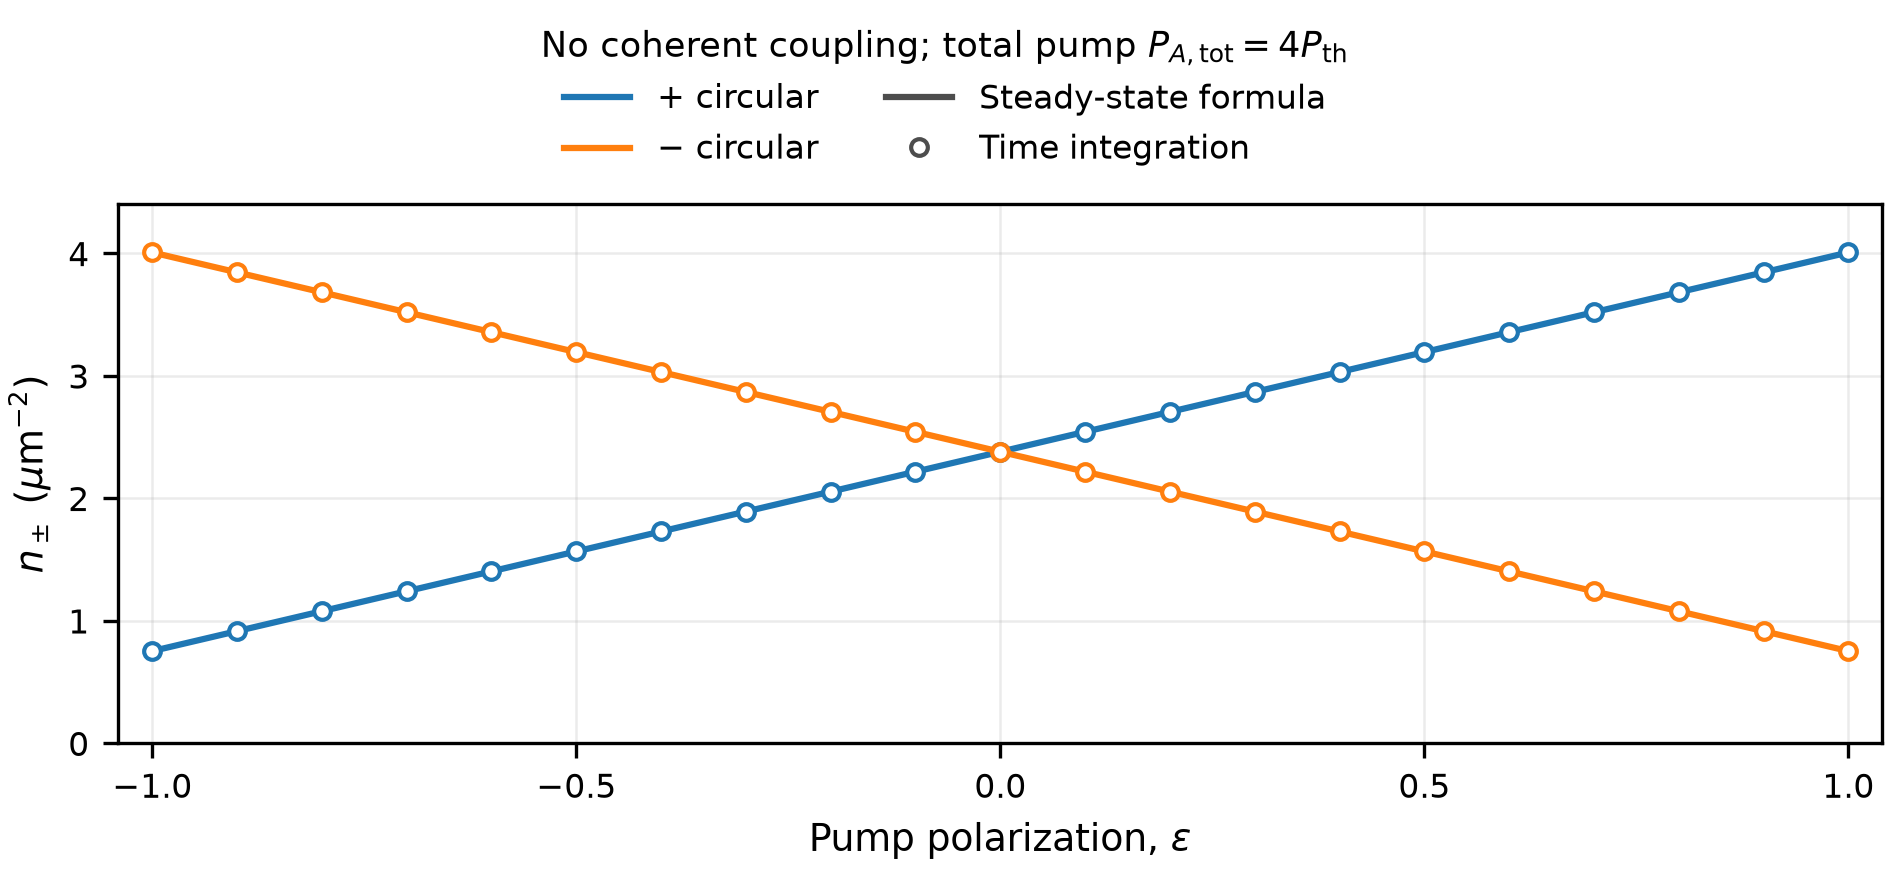
\includegraphics[width=0.96\textwidth]{../results/figures/report3/P2_homogeneous_pump_response.png}
\caption{Homogeneous steady densities versus pump polarization \(\epsilon\), at total pump \(4P_{\rm th}\) and \(J=0\), including reservoir spin relaxation. Lines show Eq. (7); circles show independent integrations. The component densities change while their sum remains constant.}
\label{fig:2}
\end{figure}

\subsection{Spatial distributions under spot and annular pumping}

The spatial calculations resolve the cavity plane, \(\mathbf r=(x,y)\). We use

\[
P_{A,\pm}(r)=pP_{\rm th}(1\pm\epsilon)f(r),
\qquad
f_{\rm spot}(r)=e^{-r^2/d^2},\qquad
f_{\rm ring}(r)=e^{-(r-r_0)^2/d^2}.
\tag{9}\label{eq:9}
\]

We use \(d=2.5\;\mu\mathrm m\), \(r_0=10\;\mu\mathrm m\), and \(p=13.8\) for the spot or \(3.3\) for the ring. Each geometry retains its pump when couplings are compared. These working points lie above the estimated spatial onsets; \(P_{\rm th}\) itself remains the homogeneous reference threshold.

Both components start with equal amplitudes and phase, and empty reservoirs. Annular runs share a weak prescribed non-axisymmetric seed perturbation (Appendix B). The main spatial comparisons use \(512^2\) points, \(L=256\;\mu\mathrm m\), and \(\Delta t=0.025\) ps. The separate high-\(J\) scan uses \(256^2\), as specified in Section 4.4. This preparation differs from the earlier report's annular series, so the old and new densities do not isolate a single changed coefficient.

Figure 3 shows the two component densities at \(\epsilon=0.3\), \(J=\beta=0\). The spot produces a central density maximum, whereas the annular pump produces an annular density distribution. The component populations differ, while their spatial profiles remain similar. We characterize them by

\[
N_\pm=\int n_\pm(\mathbf r)\,d^2r,
\qquad Z=\frac{N_+-N_-}{N_++N_-}.
\tag{10}\label{eq:10}
\]

Equation (8) does not directly determine the integrated \(Z\), because spatial transport and reservoir inhomogeneity are present. The maps show the pump-induced imbalance; they do not isolate \(\alpha_2\). Setting \(\alpha_2=0\) gives visually close profiles, but a precise small difference requires a dedicated error estimate.


\begin{figure}[H]
\centering
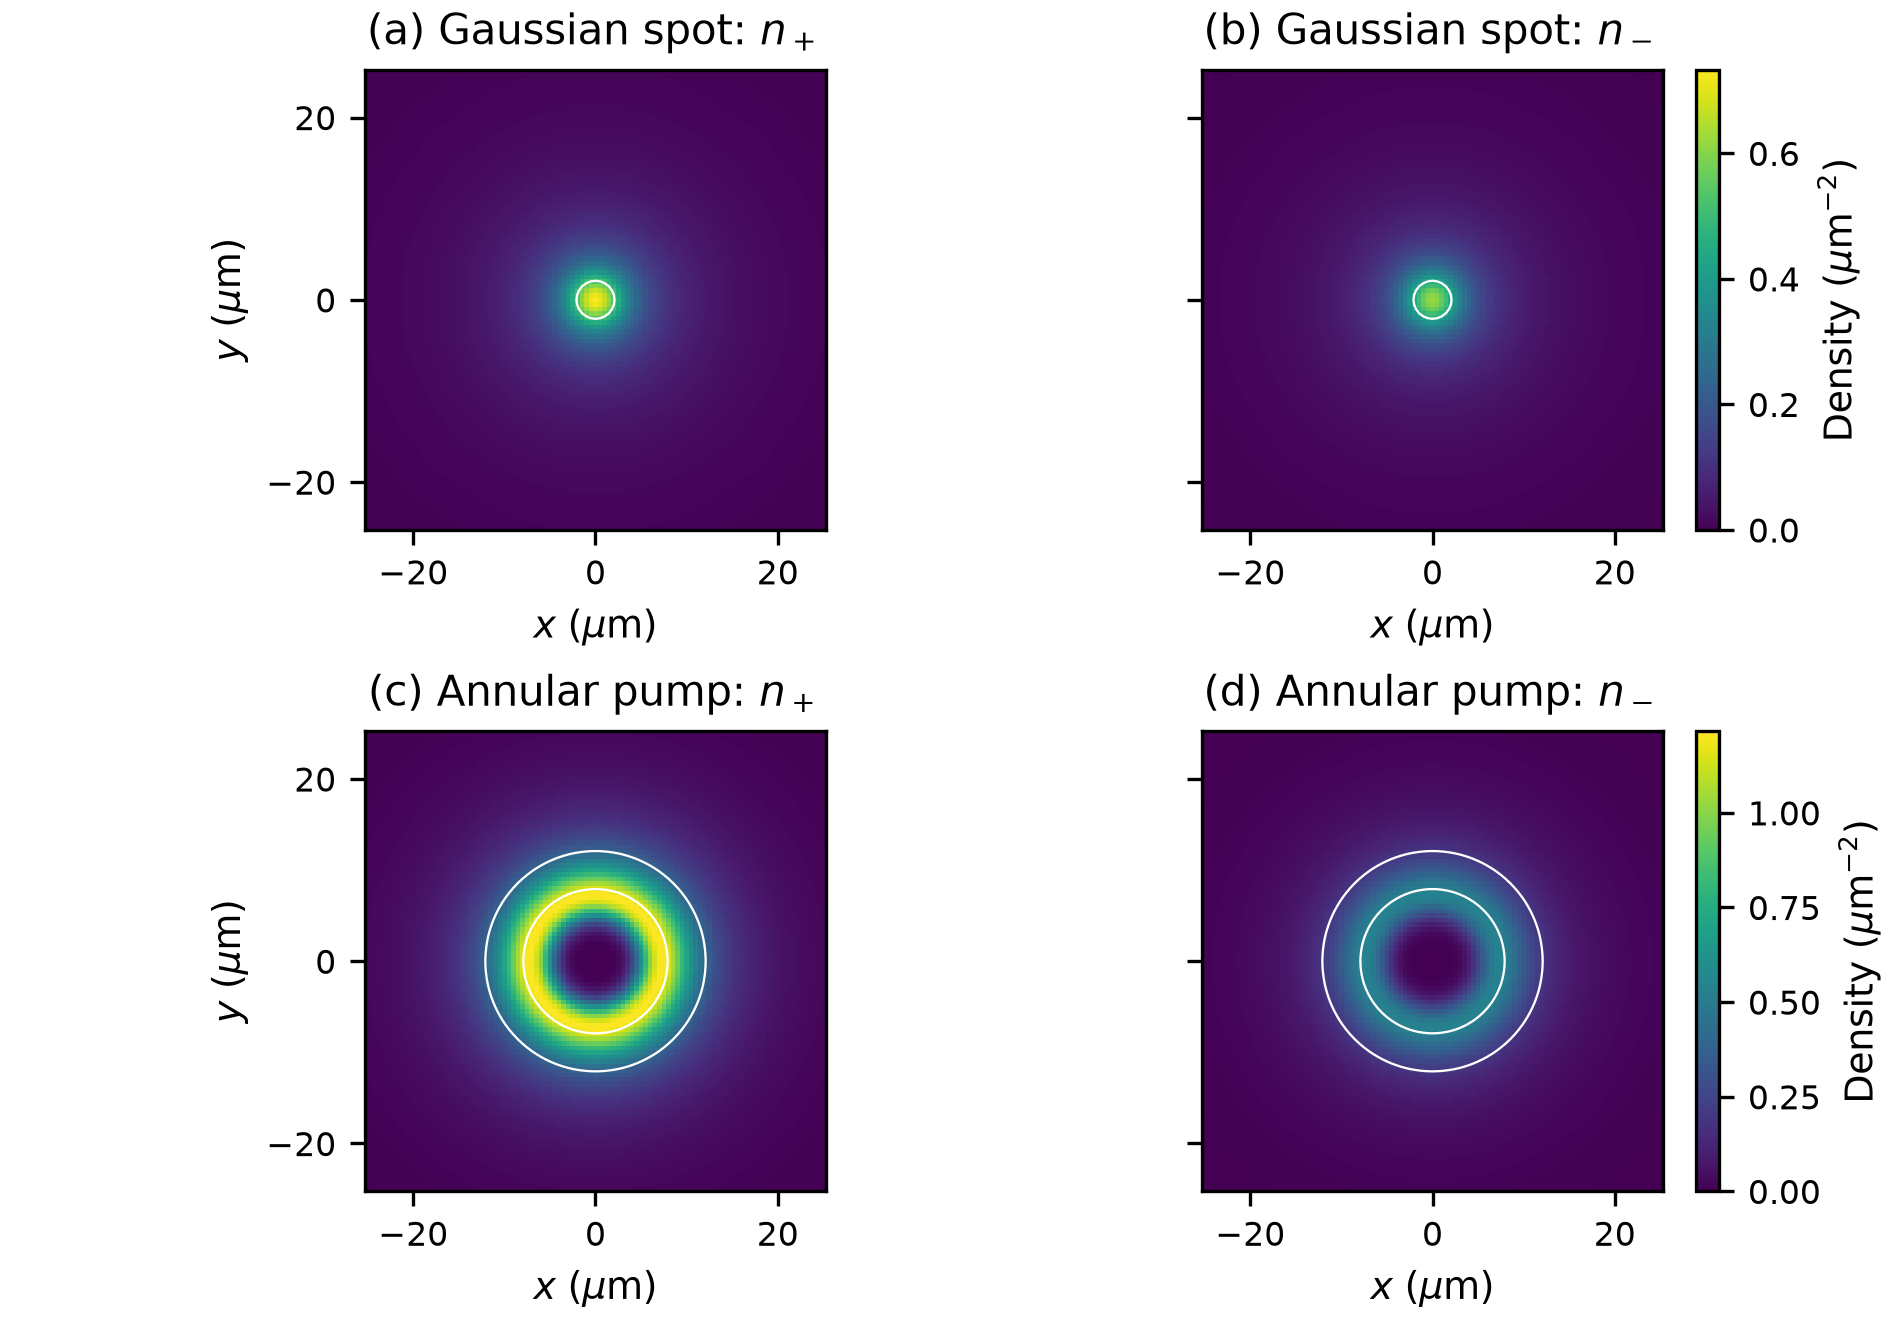
\includegraphics[width=0.96\textwidth]{../results/figures/report3/N1_spatial_component_densities.png}
\caption{Circular-component densities under Gaussian-spot (a,b) and annular (c,d) pumping, with \(\epsilon=0.3\), \(J=\beta=0\), and \(p=13.8\) and 3.3, respectively. The \(512^2\) maps show late-time density profiles; each component pair shares an absolute color scale. White contours mark half the maximum pump intensity. Sampling details are listed in Table~\ref{tab:sampling}.}
\label{fig:3}
\end{figure}

\section{Internal Josephson dynamics in the 0D model}

We now omit spatial derivatives in Eq. (5). Figures 4--6 describe independent homogeneous calculations, not a spatial average of Fig.~\ref{fig:3}.

\subsection{Coherent coupling and particle exchange}

The term \(-J\psi_{-\sigma}\) coherently couples the circular components of one condensate. For equal diagonal energies, its linearly polarized eigenstates are separated by \(2J\), independently of momentum. Internal Josephson dynamics therefore require no TE--TM splitting. Nonresonant pumping supplies reservoir particles, while the field equations determine the relative phase \cite{ref4}.

Writing \(\psi_\pm=\sqrt{n_\pm}e^{i\varphi_\pm}\), define

\[
\theta=\varphi_+-\varphi_-,\qquad
I_J=\frac{2J}{\hbar}\operatorname{Im}(\psi_-^*\psi_+)
=\frac{2J}{\hbar}\sqrt{n_+n_-}\sin\theta.
\tag{11}\label{eq:11}
\]

Positive \(I_J\) denotes transfer into the + component:

\[
\dot n_+=(Rn_{A,+}-\gamma_C)n_++I_J,\qquad
\dot n_-=(Rn_{A,-}-\gamma_C)n_--I_J.
\tag{12}\label{eq:12}
\]

The relative phase obeys

\[
\dot\theta=-\frac{V_+-V_-}{\hbar}
-\frac{2J}{\hbar}\frac{z}{\sqrt{1-z^2}}\cos\theta.
\tag{13}\label{eq:13}
\]

A fixed relative phase need not be zero: both field phases may evolve at a common rate. Spatial uniformity is assumed in this 0D model, not established by phase locking.

\subsection{Three observed dynamical regimes}

The calculations use \(s=2\), \(\epsilon=0.3\), and identical initial conditions. Three examples are retained from the previous version:

\begin{itemize}
\item At \(J=5\;\mu\mathrm{eV}\), the densities oscillate periodically and the relative phase continues to wind.
\item At \(J=6.5\;\mu\mathrm{eV}\), density oscillations persist, but the relative phase oscillates within a bounded interval.
\item At \(J=10\;\mu\mathrm{eV}\), the densities and relative phase become constant.

\end{itemize}
Figures 4 and 5 show the densities and phase over the same late-time interval. Vanishing mean phase drift does not imply that the density oscillations have ceased.

At \(J=10\;\mu\mathrm{eV}\), the steady current is \(I_J\simeq0.01477\;\mu\mathrm m^{-2}\mathrm{ps}^{-1}\). It compensates the unequal gain-loss balance of the two components. A fixed relative phase can therefore coexist with nonzero particle transfer, while the fields rotate at a common frequency.


\begin{figure}[H]
\centering
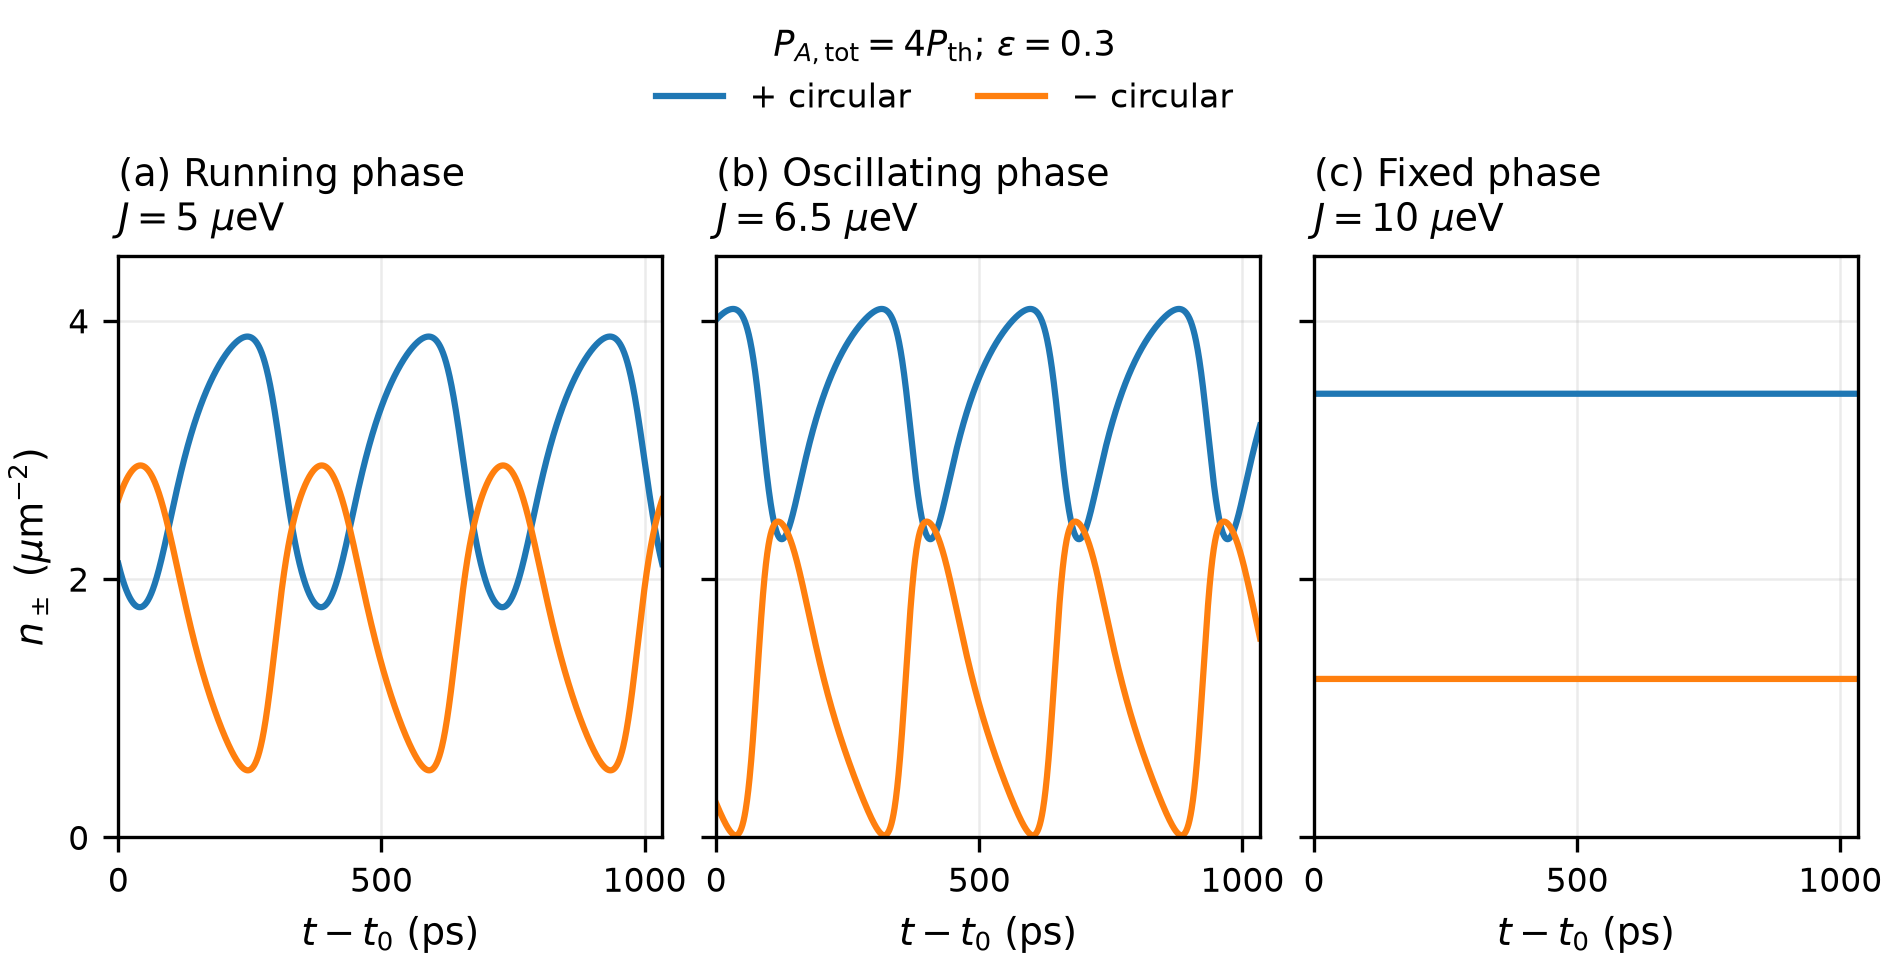
\includegraphics[width=0.96\textwidth]{../results/figures/report3/P3_homogeneous_densities.png}
\caption{Homogeneous densities at \(J=5\), 6.5, and 10 \ensuremath{\mu}eV: running phase (a), bounded phase oscillations (b), and fixed phase (c). The total pump is \(4P_{\rm th}\), with \(\epsilon=0.3\). All panels share component colors and a density scale. The interval is \(16966.5\le t\le18000\) ps, displayed relative to its start.}
\label{fig:4}
\end{figure}


\begin{figure}[H]
\centering
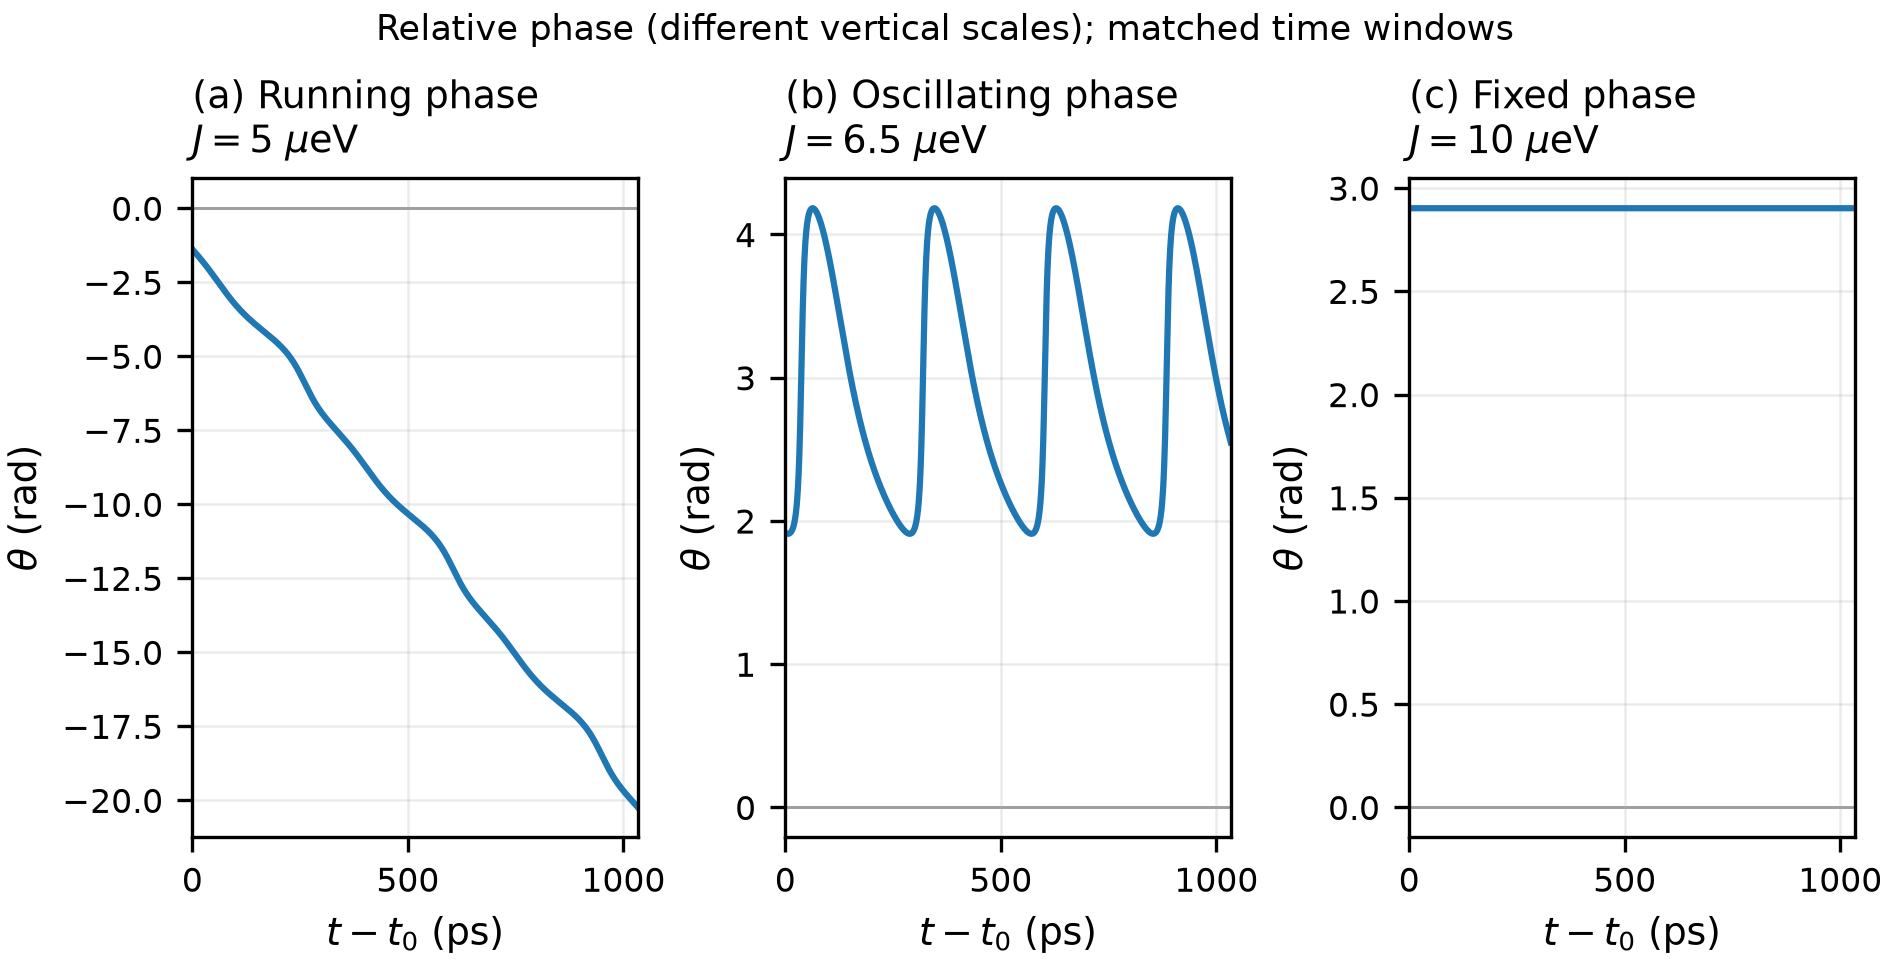
\includegraphics[width=0.96\textwidth]{../results/figures/report3/P4_homogeneous_relative_phase.png}
\caption{Unwrapped relative phase \(\theta=\arg(\psi_+\psi_-^*)\) for the calculations and interval of Fig.~\ref{fig:4}. The vertical scales differ. Only integer multiples of \(2\pi\) are subtracted, preserving the steady state's nonzero phase difference.}
\label{fig:5}
\end{figure}

\subsection{Dependence on the coupling strength}

Two quantities distinguish the regimes:

\[
A_z=\frac{z_{\max}-z_{\min}}{2},\qquad
\Omega_\theta=\langle\dot\theta\rangle.
\tag{14}\label{eq:14}
\]

Here \(A_z\) is the imbalance half-amplitude. Figure 6 plots the mean relative-phase drift \(\Omega_\theta=\langle\dot\theta\rangle\), evaluated over complete late-time cycles. With \(\theta=\arg(\psi_+\psi_-^*)\), the running-phase examples have negative drift. This is the opposite sign to the frequency difference \(\overline{\omega_+-\omega_-}\) when \(\omega_\sigma=-\partial_t\arg\psi_\sigma\).

In the retained homogeneous series, the mean phase drift vanishes near \(J=6.4\;\mu\mathrm{eV}\), while density oscillations persist to stronger coupling. Their disappearance is bracketed by the sampled values \(6.84\) and \(6.86\;\mu\mathrm{eV}\). At \(6.38\) and \(6.40\;\mu\mathrm{eV}\), one component becomes too weak during part of the cycle for its phase to be determined reliably. Density periodicity is confirmed, but no phase-drift value is assigned.

These transitions concern an existing condensate, not its condensation threshold. Independent runs with the same initial state sample one preparation protocol, rather than all possible branches.


\begin{figure}[H]
\centering
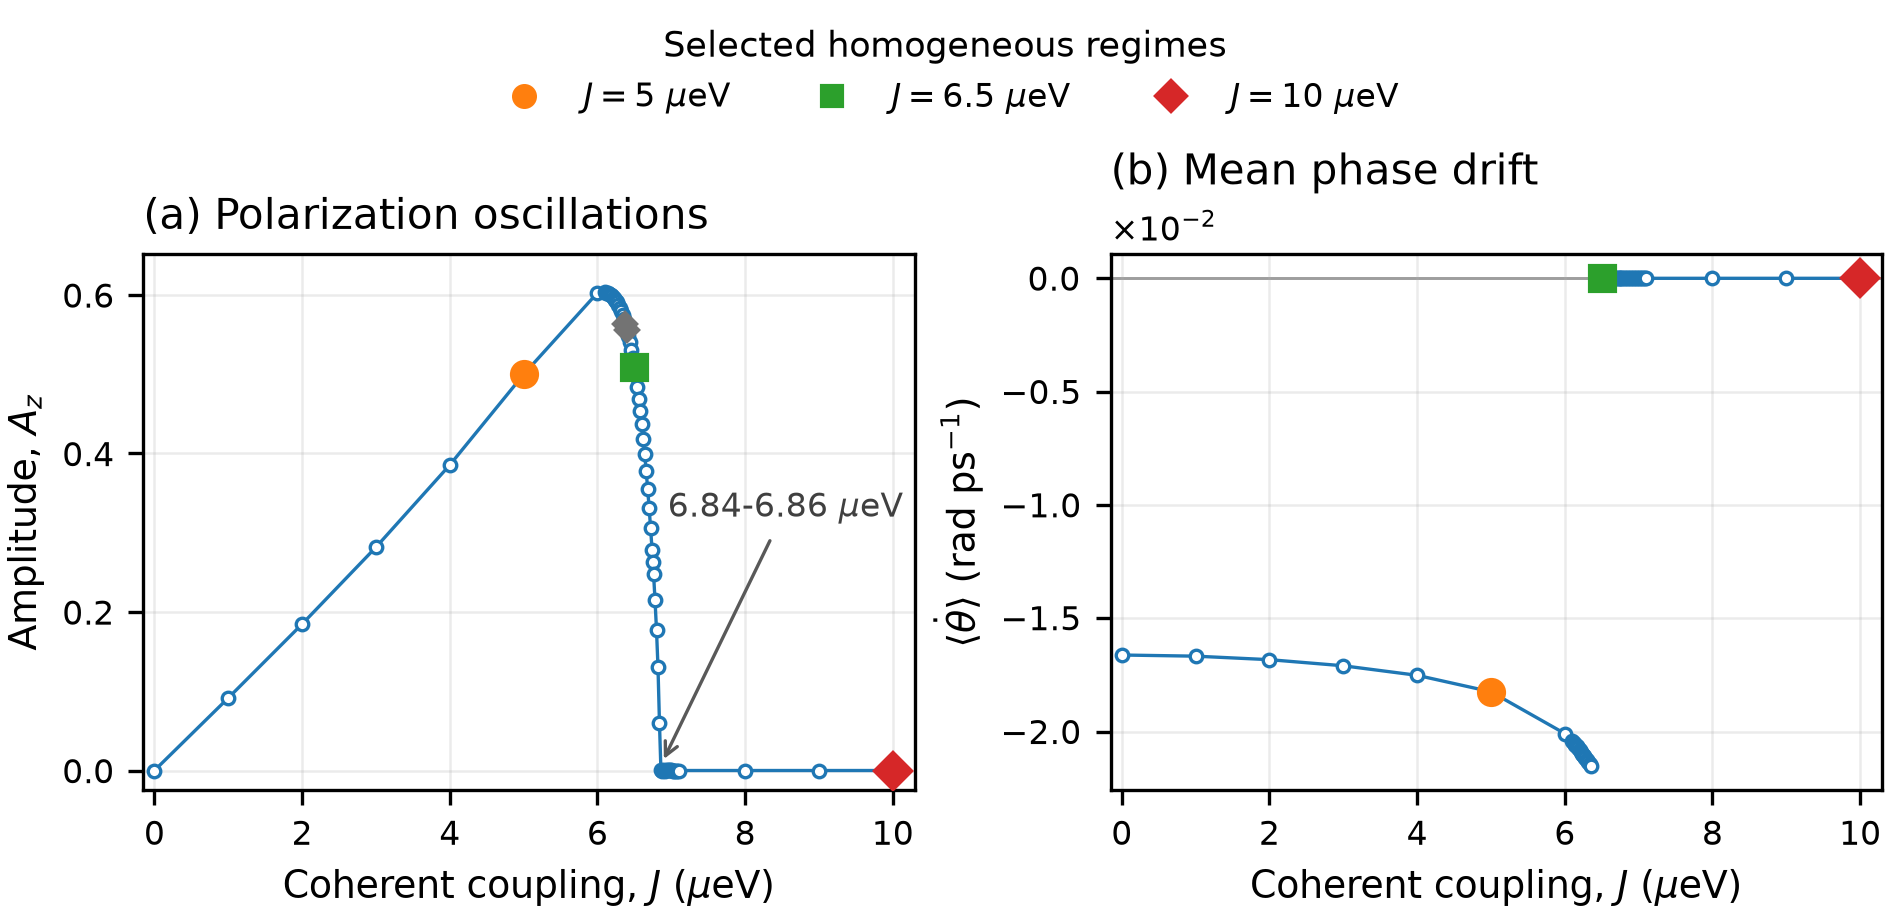
\includegraphics[width=0.96\textwidth]{../results/figures/report3/P5_homogeneous_J_scan.png}
\caption{Homogeneous coupling scan at total pump \(4P_{\rm th}\) and \(\epsilon=0.3\): imbalance half-amplitude \(A_z\) (a) and mean relative-phase drift \(\Omega_\theta=\langle\dot\theta\rangle\) (b). Oscillatory averages cover complete periods. Highlighted markers identify Figs.~\ref{fig:4}--\ref{fig:5}. Gray diamonds denote density cycles with unreliable phase near a weak component; their phase-drift values are omitted. Density oscillations disappear between the sampled 6.84 and 6.86 \ensuremath{\mu}eV points. Connecting lines guide the eye.}
\label{fig:6}
\end{figure}

\section{TE--TM splitting and spatial polarization}

\subsection{Extension of the field equations}

The two circular fields already span the lower-polariton polarization space. TE and TM are linear combinations with axes set by the in-plane propagation direction; no additional wave functions are required. Separate photon/exciton amplitudes and the upper branch are not resolved.

The field equations become

\[
i\hbar\partial_t\psi_\pm=
\left[-K\nabla^2+V_\pm+\frac{i\hbar}{2}(Rn_{A,\pm}-\gamma_C)\right]\psi_\pm
-J\psi_\mp-\beta(\partial_x\mp i\partial_y)^2\psi_\mp.
\tag{15}\label{eq:15}
\]

The reservoir equations remain those of Eq. (5). The added operator is the TE--TM coupling used in Ref. \cite{ref6}, written in our circular-basis convention. It couples polarization and spatial variation. In Fourier space, its off-diagonal entries are

\[
\beta(k_x\mp ik_y)^2=\beta k^2e^{\mp2i\varphi_k}.
\tag{16}\label{eq:16}
\]

At \(J=0\), the two linear dispersions have curvatures \(K+\beta\) and \(K-\beta\), so the TE--TM energy difference has magnitude \(2|\beta|k^2\). The mean curvature \(K\) is unchanged. The TE--TM term vanishes for a spatially uniform field, but need not vanish at the real-space center of an inhomogeneous condensate: \(\mathbf r=0\) is not \(\mathbf k=0\).

The three coefficients have distinct roles. The nonlinear term \(\alpha_2n_\mp\) changes a diagonal energy shift; \(J\) mixes the components independently of momentum; and \(\beta\) produces direction-dependent mixing. The coherent linear off-diagonal element is

\[
b(\mathbf k)=-J+\beta k^2e^{-2i\varphi_k},\qquad
|b|^2=J^2+\beta^2k^4-2J\beta k^2\cos2\varphi_k.
\tag{17}\label{eq:17}
\]

For equal diagonal energies, the splitting \(2|b|\) explains the angular dependence of the combined linear coupling. It is not the full excitation spectrum of the pumped nonlinear state.

\subsection{TE--TM coupling under equal pumping}

We first set \(\epsilon=0\), \(J=0\), and \(\beta=\beta_{\rm ref}=0.0119\;\mathrm{meV}\,\mu\mathrm m^2\). The condensate starts with equal real fields. The pump supplies populations through the reservoirs and does not impose a coherent optical phase on the condensate.

Figures 7 and 8 show the total density and the local degree of circular polarization,

\[
S_0=n_++n_-,\qquad s_3=\frac{n_+-n_-}{n_++n_-}.
\tag{18}\label{eq:18}
\]

The spot develops four sectors of alternating circular polarization, much clearer in \(s_3\) than in total density. This is consistent with Eq. (16), without assigning a topological charge to the texture.

For the annular pump, component densities have settled by 6000 ps, whereas polarization still changes slowly. This illustrates why density stationarity does not establish polarization stationarity: \(s_1\) and \(s_2\) also depend on relative phase (Chapter 5). A strong normalized signal in a dim region need not imply intense emission; density masks are applied throughout.


\begin{figure}[H]
\centering
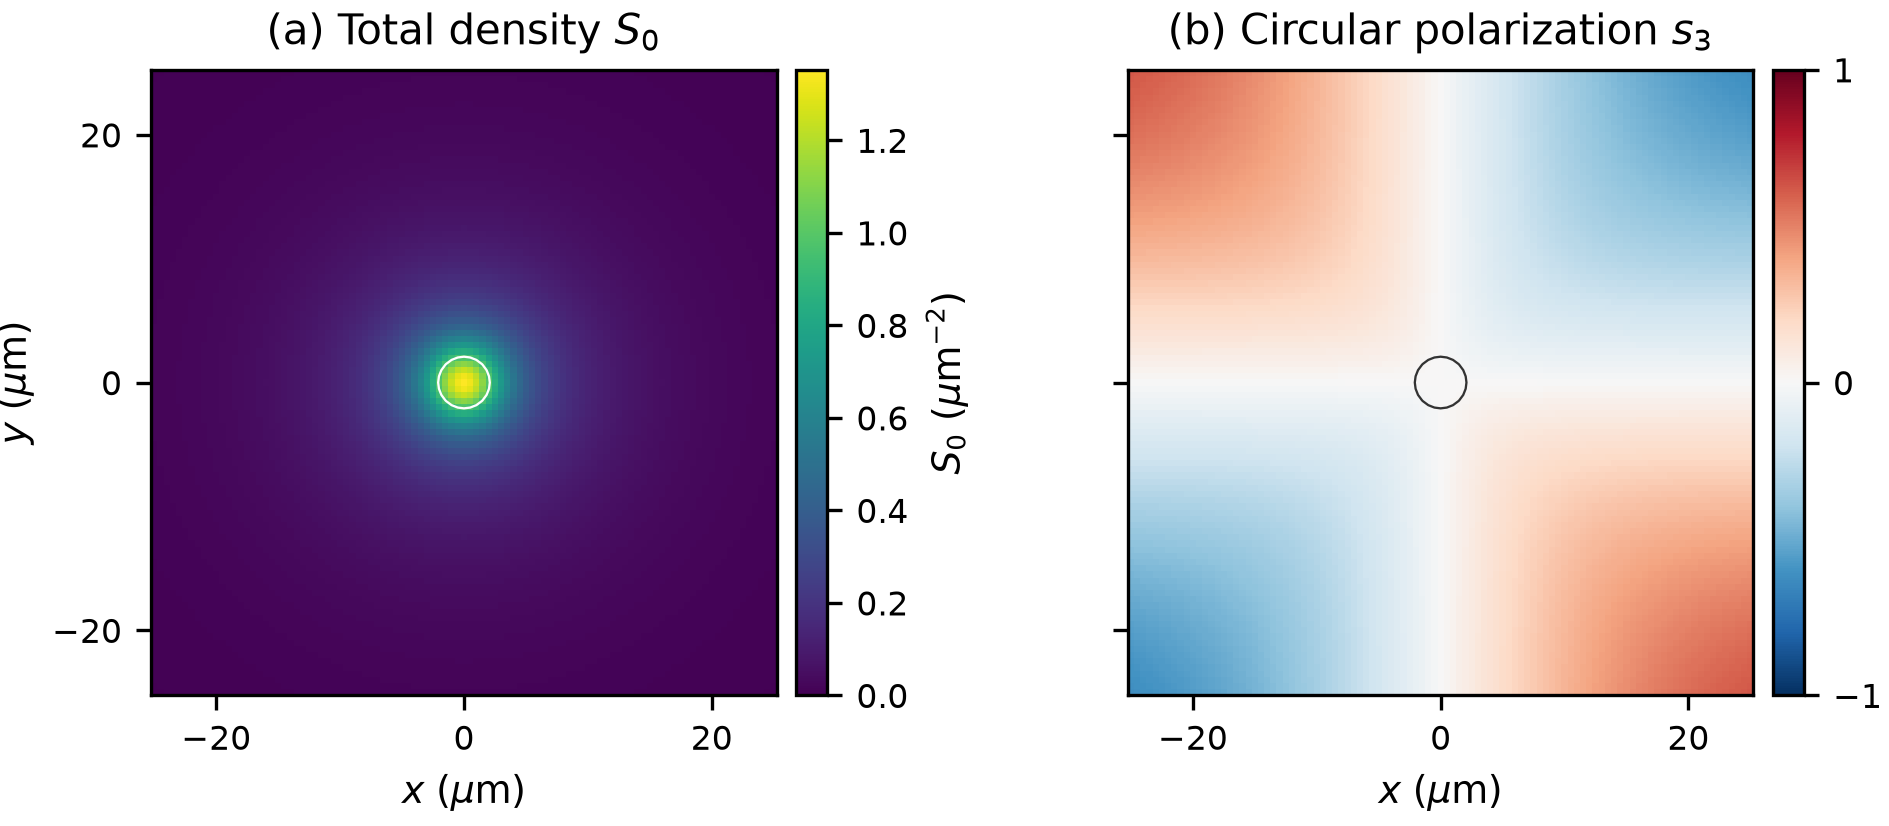
\includegraphics[width=0.96\textwidth]{../results/figures/report3/N3_TE_TM_spot.png}
\caption{Total density \(S_0\) (a) and local circular polarization \(s_3\) (b) of the Gaussian spot, with \(p=13.8\), \(\epsilon=0\), \(J=0\), and \(\beta=0.0119\) meV \ensuremath{\mu}m\textsuperscript{2}, on \(512^2\). The late-time polarization has four alternating sectors. The contour marks half the pump maximum; pixels with \(S_0<10^{-3}\max S_0\) are masked in the polarization map. Sampling details are listed in Table~\ref{tab:sampling}.}
\label{fig:7}
\end{figure}


\begin{figure}[H]
\centering
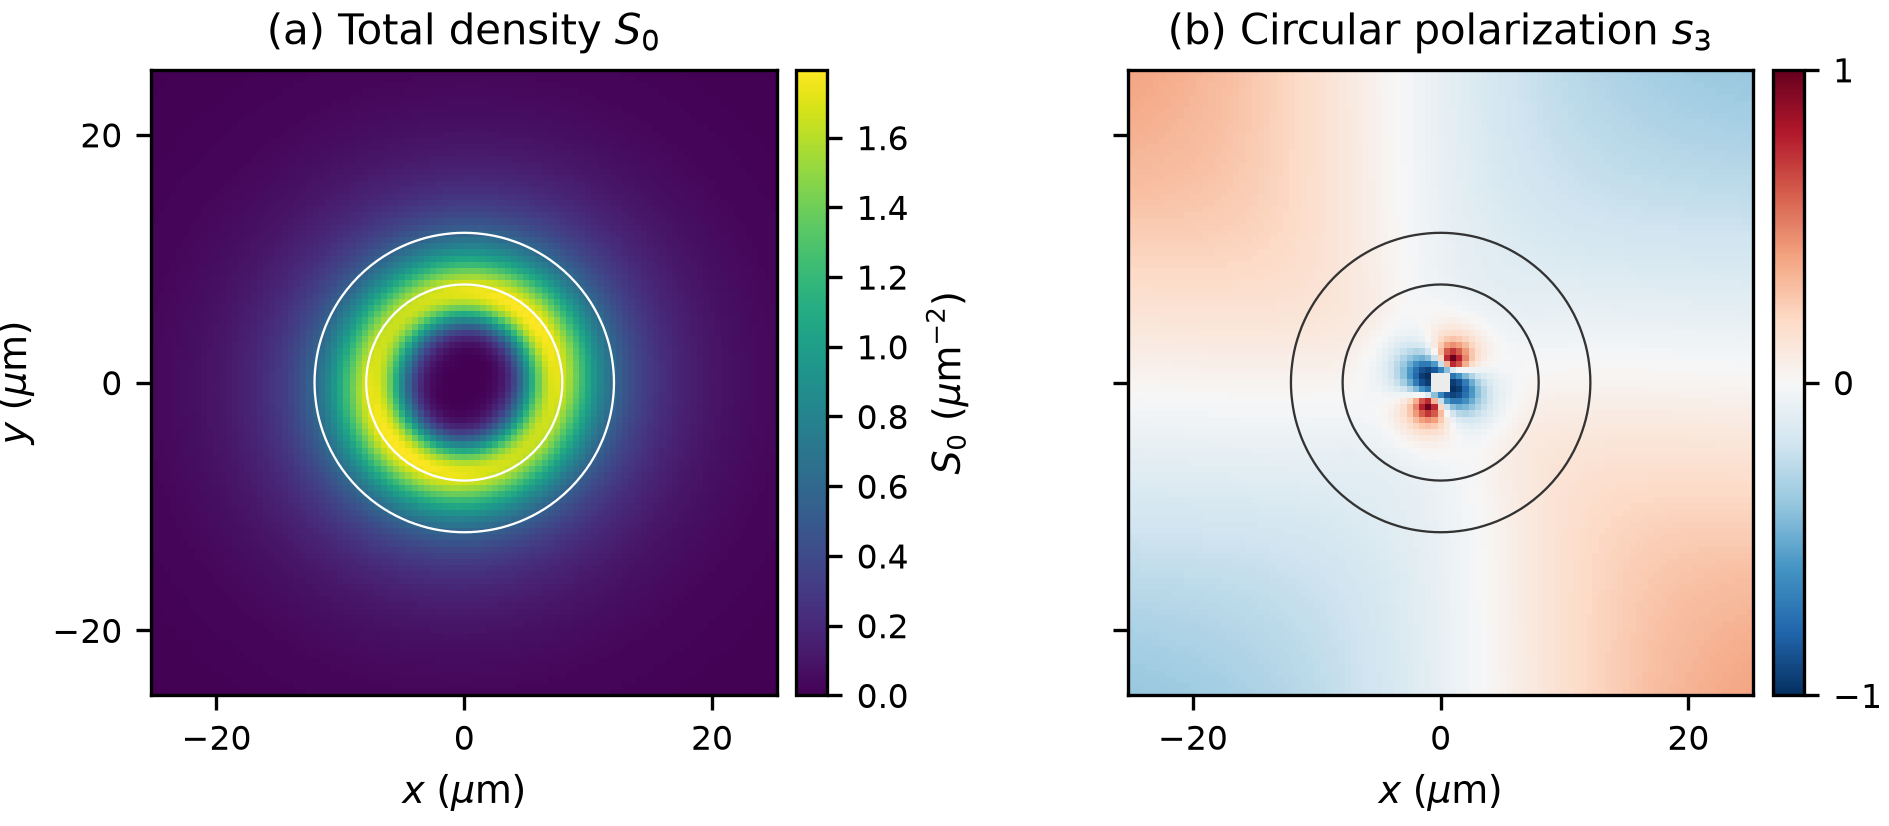
\includegraphics[width=0.96\textwidth]{../results/figures/report3/N4_TE_TM_ring.png}
\caption{Annular-pump density \(S_0\) (a) and circular polarization \(s_3\) (b) at 6000 ps, with \(p=3.3\), \(\epsilon=0\), \(J=0\), and \(\beta=0.0119\) meV \ensuremath{\mu}m\textsuperscript{2}, on \(512^2\). Densities have settled, but polarization still evolves. Circles mark half the pump maximum; the polarization mask is defined as in Fig.~\ref{fig:7}. Sampling details are listed in Table~\ref{tab:sampling}.}
\label{fig:8}
\end{figure}

To quantify the spot's angular response, define

\[
C_2(t)=\frac{\int_{\mathcal R} S_3(r,\varphi,t)e^{-2i\varphi}\,d^2r}
{\int_{\mathcal R} S_0(r,\varphi,t)\,d^2r},
\qquad Q_2(t)=2|C_2(t)|,
\qquad S_3=n_+-n_-.
\tag{19}\label{eq:19}
\]

All coefficients use the analysis annulus \(\mathcal R=\{5\le r\le15\;\mu\mathrm m\}\) and the same quadrature. The final-400-ps means of \(Q_2\) are approximately 0.0768, 0.1529, and 0.3008 for \(\beta/\beta_{\rm ref}=0.5,1,2\), with zero for the symmetric uncoupled control (Fig.~\ref{fig:9}). This nearly linear dependence describes the second harmonic over the sampled range. The varied coefficients test model sensitivity, not experimental uncertainty.


\begin{figure}[H]
\centering
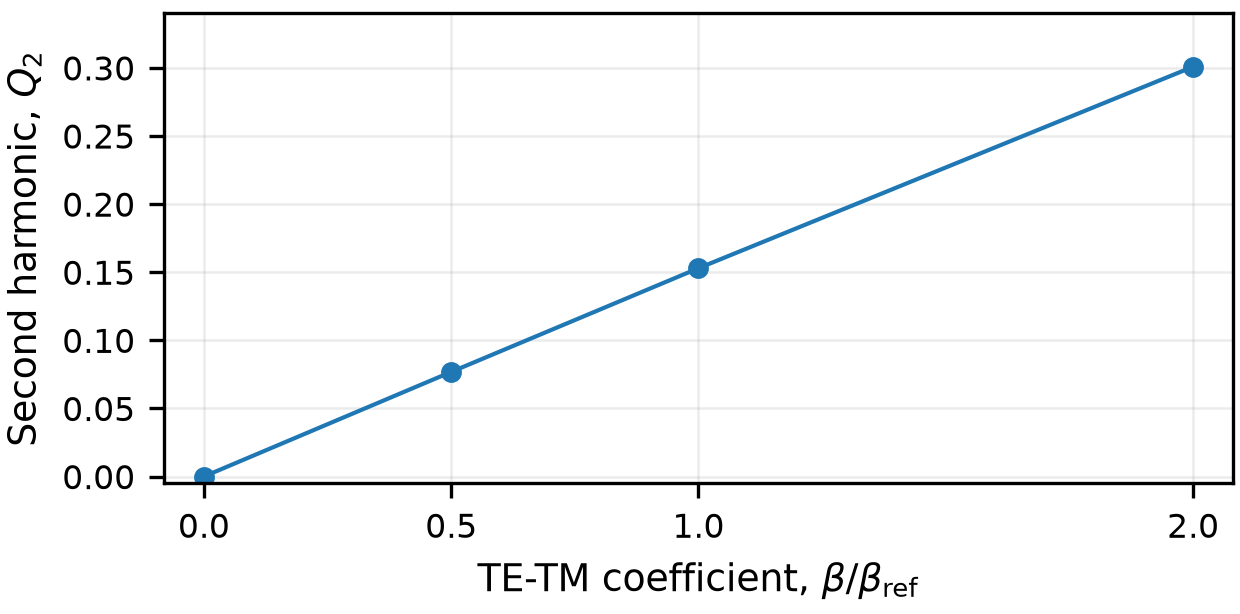
\includegraphics[width=105mm]{../results/figures/report3/N5_TE_TM_angular_response.png}
\caption{Second angular harmonic \(Q_2=2|C_2|\), defined in Eq. (19), versus TE--TM strength for the Gaussian spot. All runs use \(p=13.8\), \(\epsilon=0\), \(J=0\), \(512^2\), and the analysis annulus \(5\le r\le15\;\mu\mathrm m\) with common quadrature. Each point is the mean of \(Q_2(t)\) over 2600--3000 ps, not the modulus of averaged \(C_2\). Bars show the temporal range, not numerical uncertainty. Here \(\beta_{\rm ref}=0.0119\) meV \ensuremath{\mu}m\textsuperscript{2}; lines guide the eye. Sampling details are listed in Table~\ref{tab:sampling}.}
\label{fig:9}
\end{figure}

\subsection{Combined coupling in the annular condensate}

For the ring at \(\epsilon=0.3\), we compare no coherent coupling, TE--TM alone, \(J\) alone, and both together. Nonzero values are \(J=10\;\mu\mathrm{eV}\) and \(\beta=\beta_{\rm ref}\); other parameters and preparation are unchanged.

Figure 10 shows

\[
s_3(\varphi,t)=
\frac{\int_{r_1}^{r_2}S_3(r,\varphi,t)r\,dr}
{\int_{r_1}^{r_2}S_0(r,\varphi,t)r\,dr}.
\tag{20}\label{eq:20}
\]

This is a density-weighted radial polarization profile, not an unweighted average of local \(s_3\). All cases use \(r_1=5\;\mu\mathrm m\) and \(r_2=7.5\;\mu\mathrm m\).

The controls without TE--TM are nearly angle-independent. TE--TM alone gives four maxima per revolution; combined coupling gives two and changes the mean polarization. The former profile is an instantaneous sample of periodic dynamics, whereas the combined state is stationary within tolerance. These conclusions concern the selected states, not every preparation or time.

The combined-coupling reference has independent time-step and grid checks. Halving the step changes the late-time ring density maps by at most 0.001217\%, with a maximum RMS difference of \(4.44\times10^{-7}\) in normalized Stokes parameters. The corresponding spot reference has differences of 0.04124\% and \(8.25\times10^{-4}\), and its full-map period changes by approximately 0.00355\%. These comparisons quantify the tested reference calculations; they are not error bars for every angular profile or for the high-\(J\) scan below. Appendix B describes the common-grid comparisons and domain checks.


\begin{figure}[H]
\centering
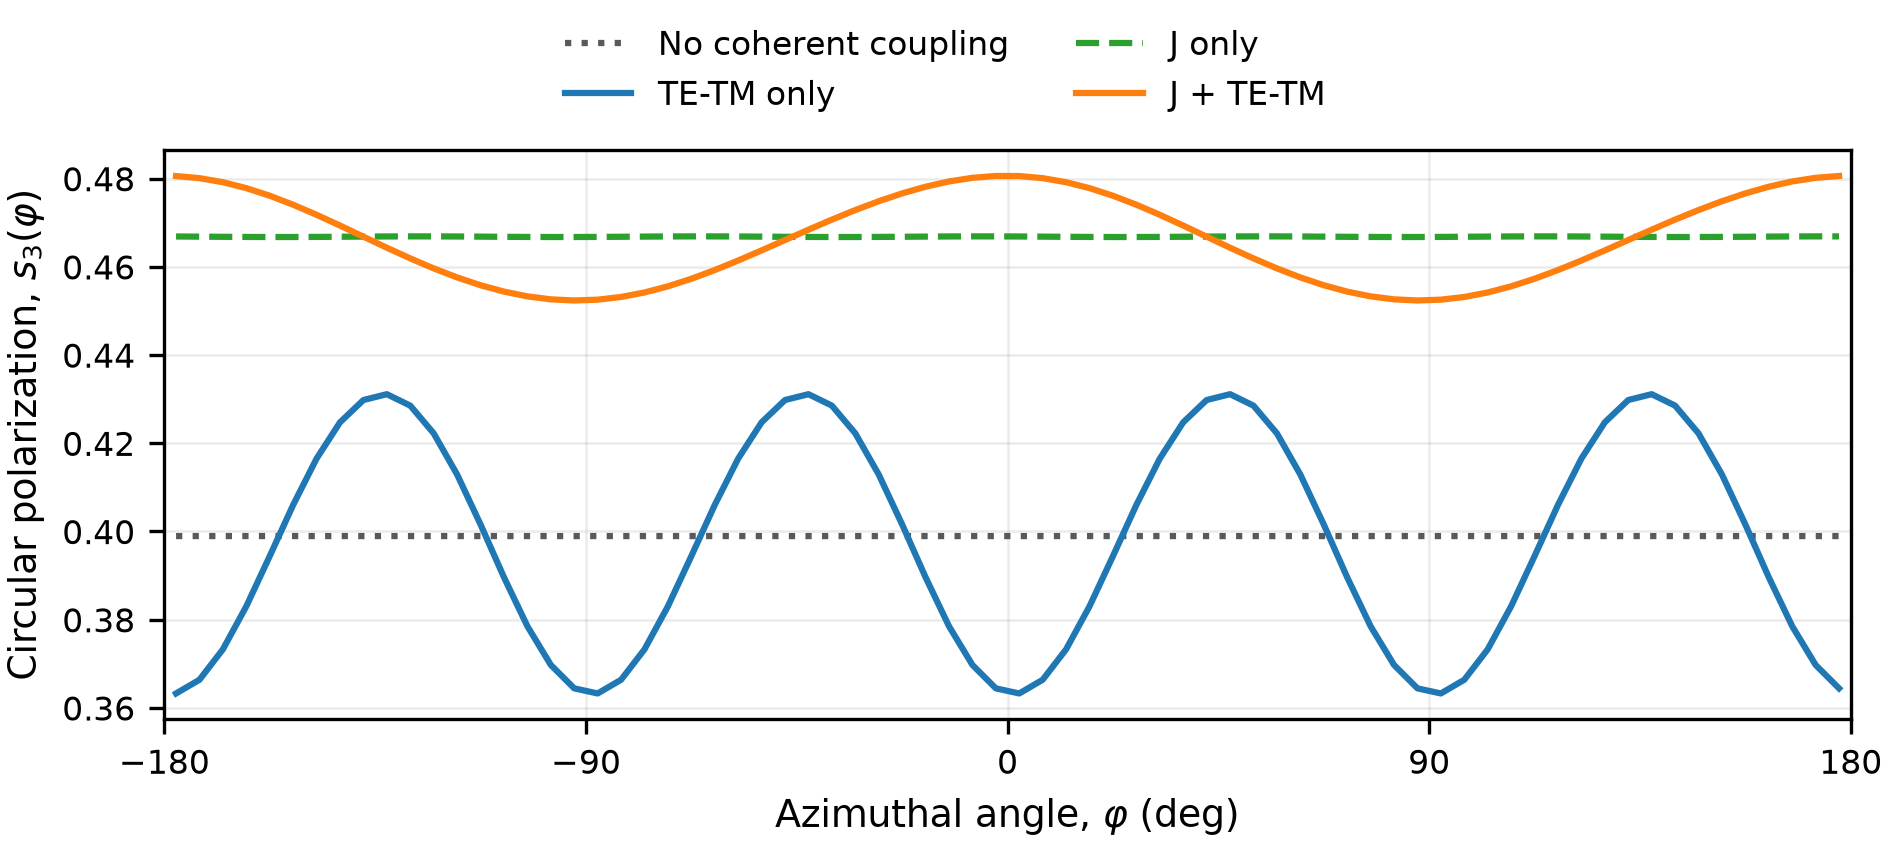
\includegraphics[width=0.96\textwidth]{../results/figures/report3/N7_ring_angular_polarization.png}
\caption{Radially weighted circular-polarization profiles, Eq. (20), for the annular condensate with neither coherent coupling, TE--TM alone, \(J\) alone, and both. Nonzero values are \(J=10\) \ensuremath{\mu}eV and \(\beta=0.0119\) meV \ensuremath{\mu}m\textsuperscript{2}; \(p=3.3\), \(\epsilon=0.3\), and the \(512^2\) grid are common. All profiles use \(5\le r\le7.5\;\mu\mathrm m\) and a common 72-sector polar Gauss quadrature. The sampling times differ between runs (Table~\ref{tab:sampling}); no common-time convergence is implied. The TE--TM-only curve is an instantaneous periodic-state profile; the combined state is stationary. Sampling details are listed in Table~\ref{tab:sampling}.}
\label{fig:10}
\end{figure}

\subsection{Three dynamical regimes of the Gaussian spot}

The spatial scan varies \(J\) at fixed \(p=13.8\), \(\epsilon=0.3\), and \(\beta=\beta_{\rm ref}\). Every run starts from the same prescribed seed; neighboring values of \(J\) are not obtained by continuing the previous final state.

The integrated observables are

\[
A_Z=\frac{Z_{\max}-Z_{\min}}{2},\qquad
\Theta(t)=\arg\!\int\psi_+(\mathbf r,t)\psi_-^*(\mathbf r,t)\,d^2r,
\qquad \Omega_\Theta=\langle\dot\Theta\rangle.
\tag{21}\label{eq:21}
\]

Unwrapping requires nonvanishing coherence. Since spatial cancellation can separate \(\Theta\) from local phase behavior, classification also uses the center and \((\pm2,0)\), \((0,\pm2)\;\mu\mathrm m\), together with density and Stokes-map recurrence.

The selected examples are \(J=40\), \(65\), and \(100\;\mu\mathrm{eV}\): running phase, bounded phase oscillations, and fixed phase, respectively (Figs.~\ref{fig:11}--\ref{fig:12}). The additional 45 \ensuremath{\mu}eV point has a running phase, 50 \ensuremath{\mu}eV remains unresolved, and 70 \ensuremath{\mu}eV has bounded phase oscillations. The confirmed samples place the running-to-bounded change between 45 and 60 \ensuremath{\mu}eV, with unresolved points inside that interval, and the bounded-to-fixed change between 70 and 75 \ensuremath{\mu}eV. These are sampled brackets for this preparation, not precise or grid-converged bifurcation values. At 55 \ensuremath{\mu}eV, periodic maps coexist with ambiguous local phase near deep component minima, so the phase classification remains unresolved. The 75 \ensuremath{\mu}eV state required extension to 4500 ps before stationarity was accepted.

The scan and the three central examples use \(256^2\), \(L=256\;\mu\mathrm m\), and \(\Delta t=0.025\) ps in double precision. Selected scan points have finer-grid, smaller-step, and larger-domain controls; the 40, 65, and 100 \ensuremath{\mu}eV examples do not all have independent \(512^2\) checks. Their observed regimes are reported at this resolution, without assigning grid-converged transition values. The stronger couplings than in 0D cannot be attributed to TE--TM alone: pump strength, transport, and reservoir profiles also differ.

Figure 12 shows central imbalance and unwrapped relative phase. The local polarization periods, denoted consistently by \(T_c\), are 34.6402 ps at 40 \ensuremath{\mu}eV and 25.0861 ps at 65 \ensuremath{\mu}eV; the 100 \ensuremath{\mu}eV example is stationary. These values are confirmed local return times, not proven minimal periods or uncertainty bounds. They are half the periods selected by the earlier full-map analyzer. Local Stokes return errors are approximately \(2.74\times10^{-4}\) and \(1.53\times10^{-6}\), respectively, and the temporal-interpolation cross-check also passes. Central trajectories and full spatial maps remain different observables; a local return does not establish recurrence of the entire pattern.


\begin{figure}[H]
\centering
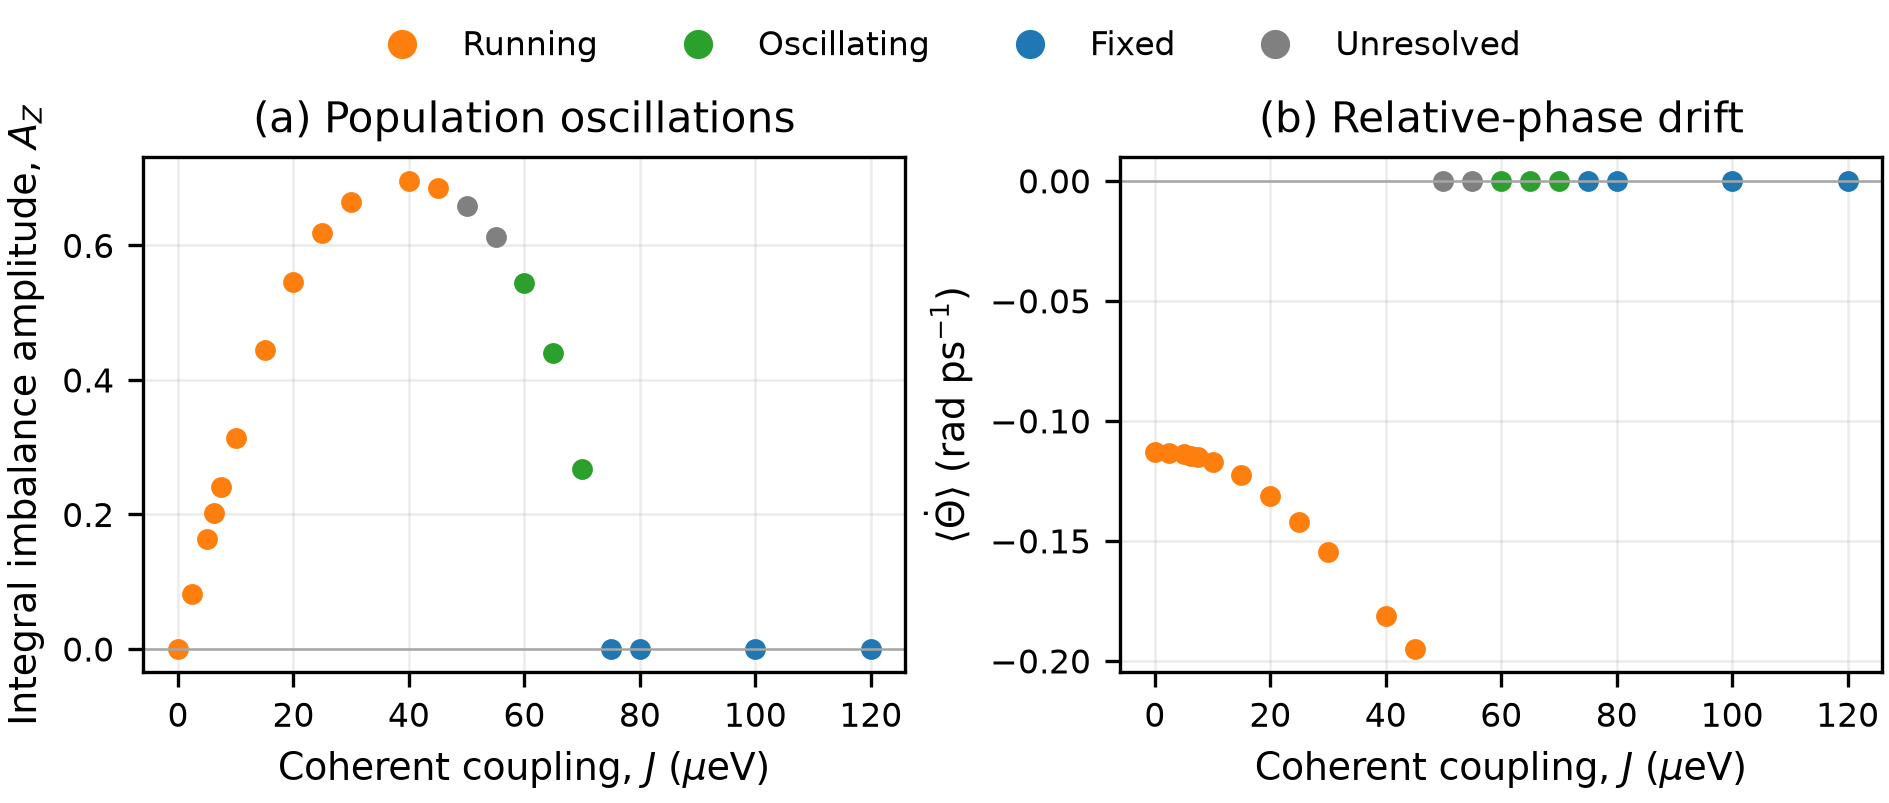
\includegraphics[width=0.96\textwidth]{../results/figures/report3/N12_spot_J_scan.png}
\caption{Gaussian-spot coupling scan at \(\beta=0.0119\) meV \ensuremath{\mu}m\textsuperscript{2}, \(p=13.8\), and \(\epsilon=0.3\): integrated imbalance half-amplitude \(A_Z\) (a) and integrated-coherence phase drift \(\Omega_\Theta\) (b), defined in Eq. (21). Colors distinguish running, bounded oscillating, fixed, and unresolved phase classifications, with local phase checks. Each point starts independently. The main scan uses \(256^2\), with selected numerical controls; precise transition boundaries are not established.}
\label{fig:11}
\end{figure}


\begin{figure}[H]
\centering
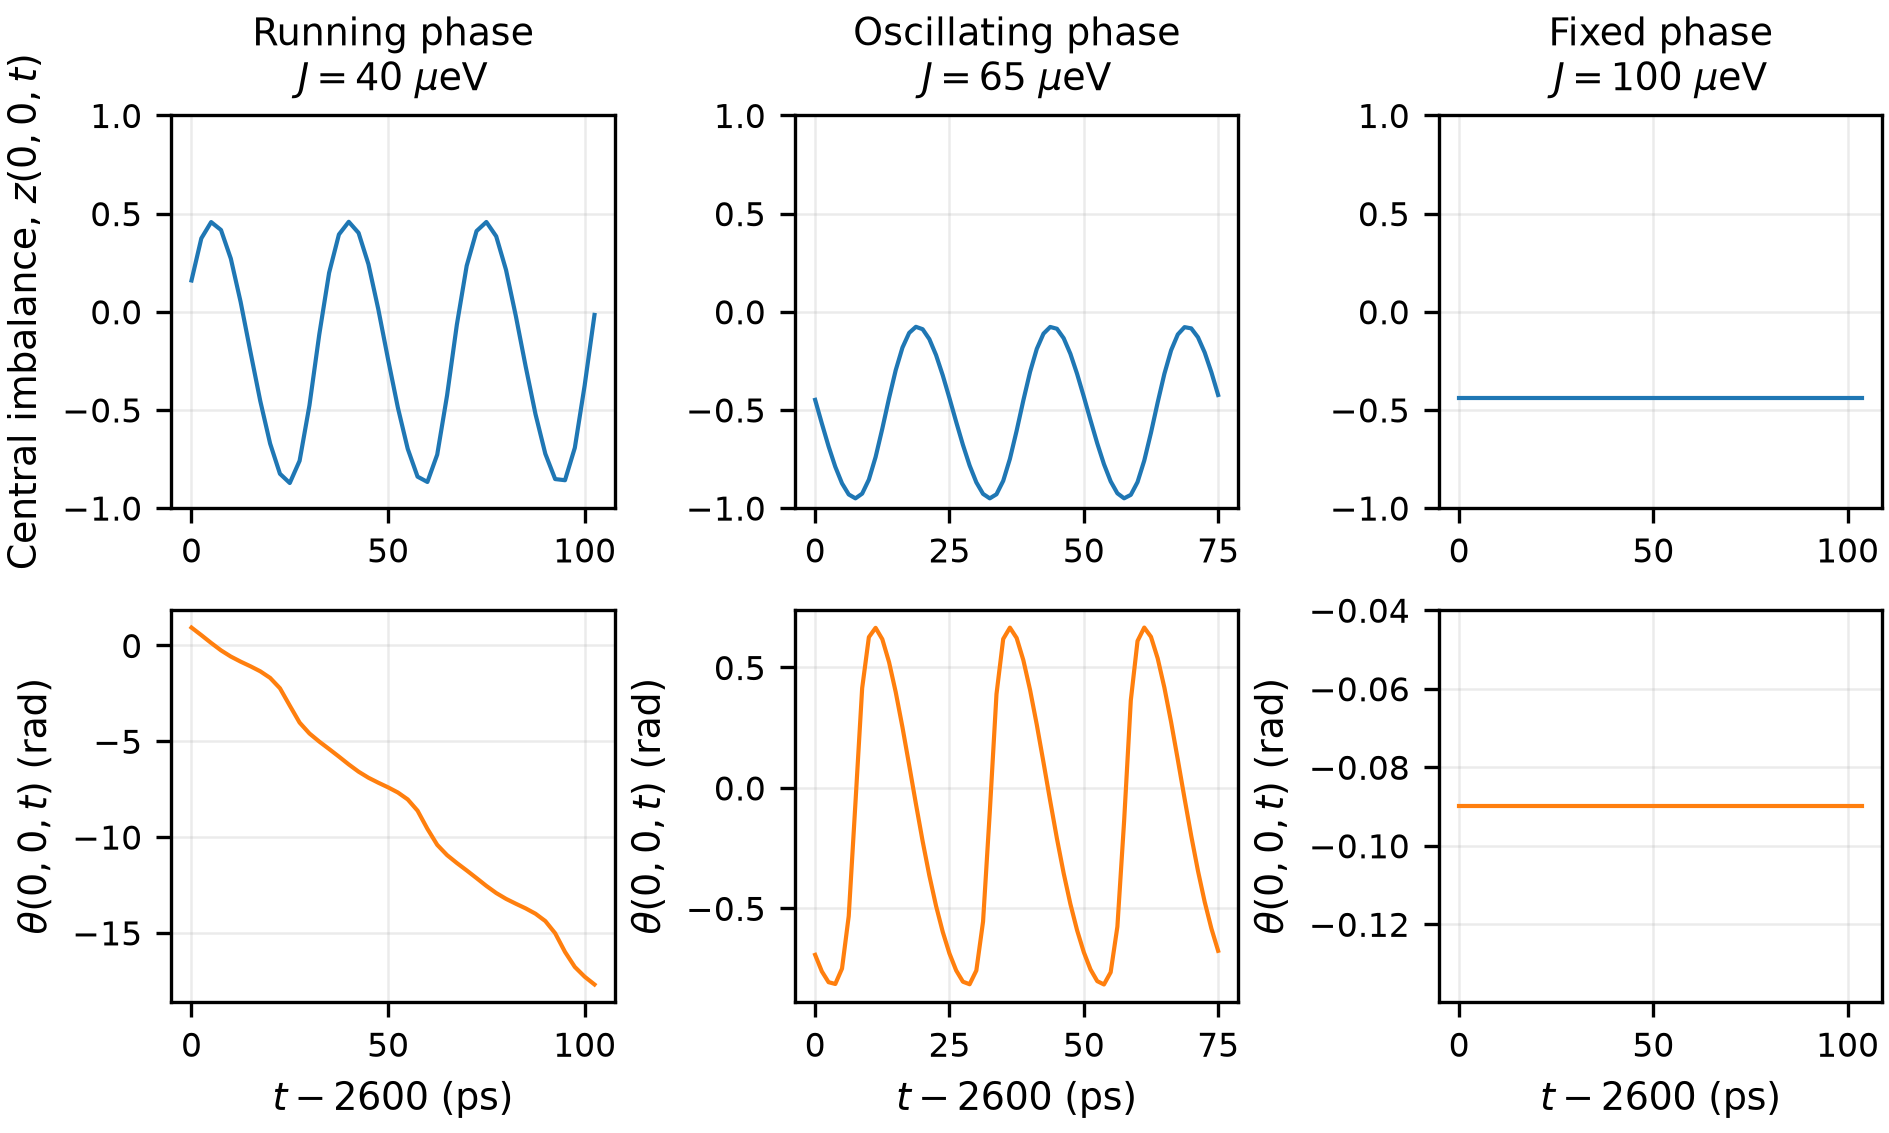
\includegraphics[width=0.96\textwidth]{../results/figures/report3/N13_spot_regime_dynamics.png}
\caption{Central dynamics of the 2D Gaussian spot at \(J=40\), 65, and 100 \ensuremath{\mu}eV: running phase (a), bounded phase oscillations (b), and fixed phase (c). Top: local imbalance \(z(0,0,t)\). Bottom: unwrapped local phase \(\theta(0,0,t)\). All cases use \(p=13.8\), \(\epsilon=0.3\), \(\beta=0.0119\) meV \ensuremath{\mu}m\textsuperscript{2}, and \(256^2\). All panels use \(t-t_0\), with the common start \(t_0=2600\) ps. Local polarization periods are approximately 34.6402 and 25.0861 ps in (a,b); the nonzero fixed phase in (c) is retained. Sampling details are listed in Table~\ref{tab:sampling}.}
\label{fig:12}
\end{figure}

\section{Stokes parameters and the Poincaré sphere}

\subsection{Definitions and normalization}

The component densities determine circular polarization, but they do not specify the full polarization state. The relative phase is also required. For the circular basis \(\mathbf e_\pm=(\mathbf e_x\pm i\mathbf e_y)/\sqrt2\), we define

\[
\begin{aligned}
S_0&=|\psi_+|^2+|\psi_-|^2,\\
S_1&=2\operatorname{Re}(\psi_+^*\psi_-),\qquad
S_2=2\operatorname{Im}(\psi_+^*\psi_-),\\
S_3&=|\psi_+|^2-|\psi_-|^2,\qquad s_i=S_i/S_0.
\end{aligned}
\tag{22}\label{eq:22}
\]

\(S_i\) have density units; \(s_i\) are dimensionless and normalized by the density at the same position and time, not the image maximum. They describe H/V, ±45°, and circular polarization with signs fixed by the stated basis.

For a coherent two-component field at a point with \(S_0>0\),

\[
\mathbf s=\left(\sqrt{1-z^2}\cos\theta,
-\sqrt{1-z^2}\sin\theta,z\right),
\qquad s_1^2+s_2^2+s_3^2=1.
\tag{23}\label{eq:23}
\]

The instantaneous local state lies on the unit Poincaré sphere: the poles represent circular and the equator linear polarization. The axes label polarization states, not directions of particle motion.

For an unresolved spatial or temporal measurement, average \(S_i\) first and divide by averaged \(S_0\). Cancellation can place this vector inside the sphere; it must not be forced back to unit length. The trajectories below instead use instantaneous local fields.

\subsection{Spatial polarization maps}

Figures 13--14 show simultaneous maps of all three normalized Stokes parameters. Equal component densities imply \(s_3=0\), while phase variation can still produce structure in \(s_1,s_2\). Round density profiles therefore need not have uniform polarization.

The spot map uses the selected running-phase calculation at \(J=40\;\mu\mathrm{eV}\), on \(256^2\); its center provides the corresponding trajectory in Fig.~\ref{fig:16}. The ring uses the stationary combined-coupling reference at \(J=10\;\mu\mathrm{eV}\), on \(512^2\). These are illustrations of different states, not a controlled comparison at equal pump and coupling.


\begin{figure}[H]
\centering
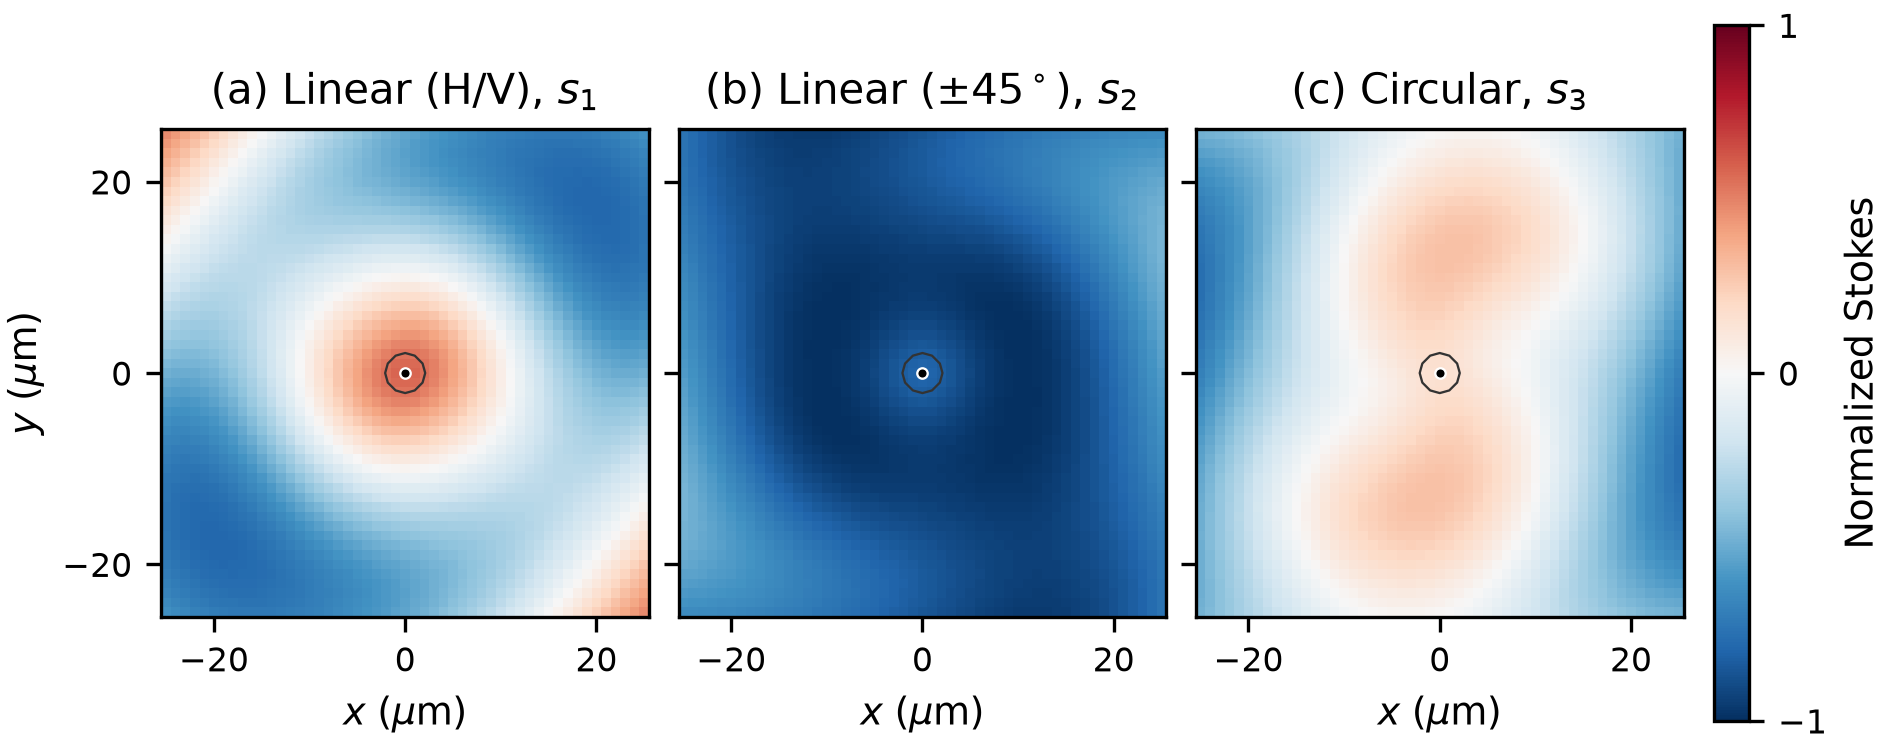
\includegraphics[width=0.96\textwidth]{../results/figures/report3/N8_spot_Stokes.png}
\caption{Instantaneous normalized Stokes maps of the running-phase Gaussian spot at \(J=40\) \ensuremath{\mu}eV: H/V polarization \(s_1\) (a), ±45° polarization \(s_2\) (b), and circular polarization \(s_3\) (c). Parameters and \(256^2\) grid match Fig.~\ref{fig:12}(a). Panels show \(t=2600\) ps with the common scale \([-1,1]\); normalization is local. The contour marks half the pump maximum, and the dot marks the center. The density mask follows Fig.~\ref{fig:7}. Sampling details are listed in Table~\ref{tab:sampling}.}
\label{fig:13}
\end{figure}


\begin{figure}[H]
\centering
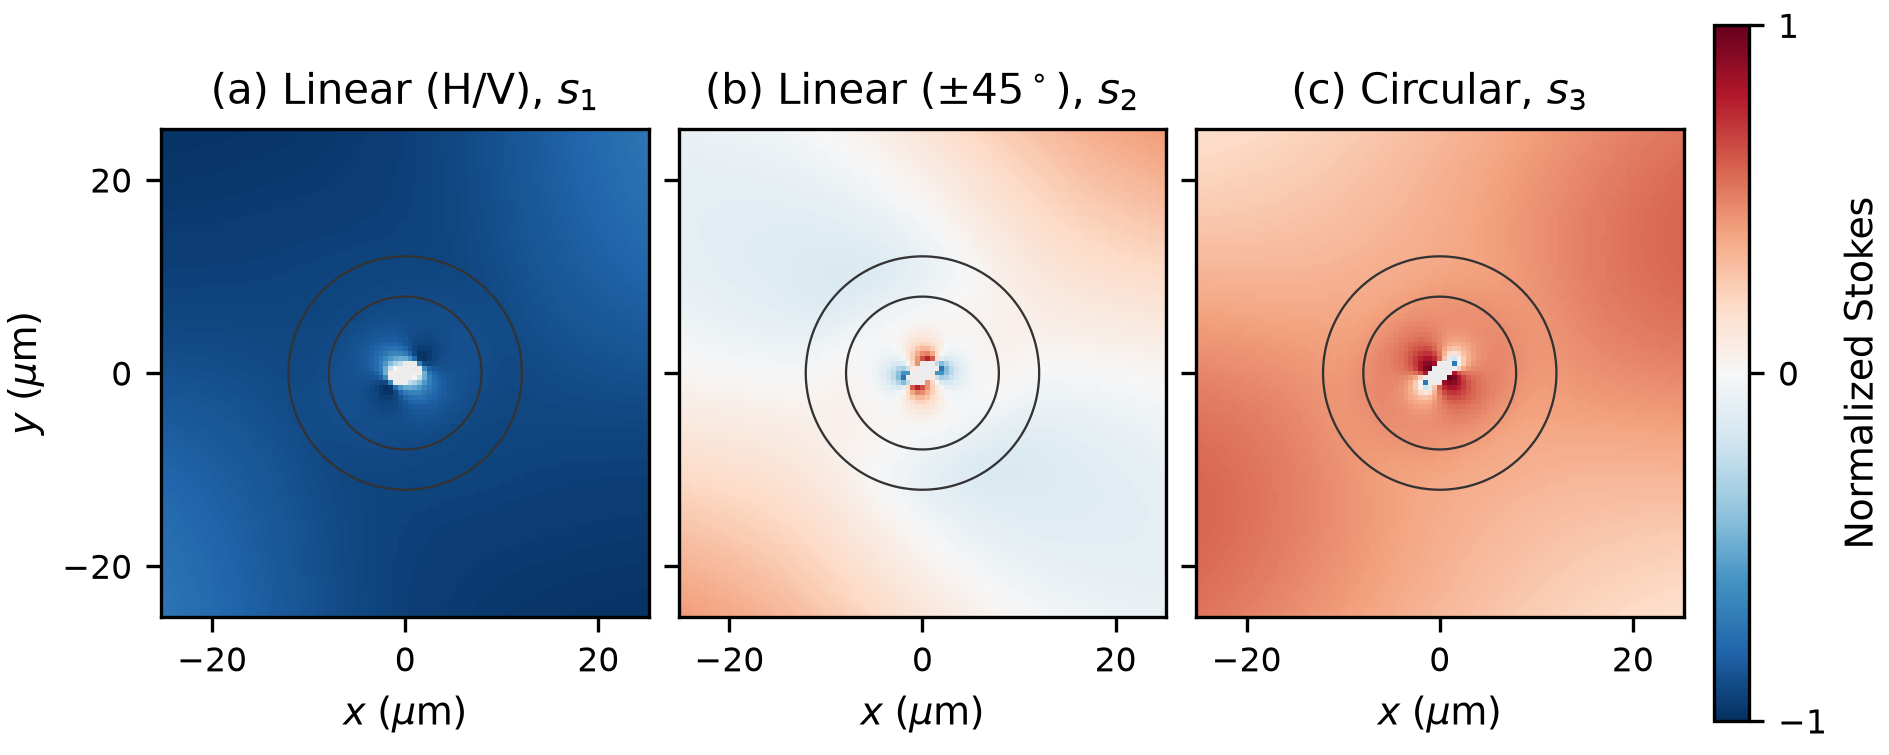
\includegraphics[width=0.96\textwidth]{../results/figures/report3/N9_ring_Stokes.png}
\caption{Normalized Stokes maps of the stationary annular reference: \(s_1\) (a), \(s_2\) (b), and \(s_3\) (c), at \(J=10\) \ensuremath{\mu}eV, \(\beta=0.0119\) meV \ensuremath{\mu}m\textsuperscript{2}, \(p=3.3\), and \(\epsilon=0.3\), on \(512^2\). Panels show \(t=3600\) ps with the common scale \([-1,1]\). Circles mark half the pump maximum; the density mask follows Fig.~\ref{fig:7}. Sampling details are listed in Table~\ref{tab:sampling}.}
\label{fig:14}
\end{figure}

\subsection{The three homogeneous regimes on the sphere}

Figure 15 represents the same 0D solutions as Figs.~\ref{fig:4}--\ref{fig:5}. Running and bounded phase oscillations both form closed polarization paths; the fixed-phase state is a point.

A closed path does not imply a bounded unwrapped phase: a \(2\pi\) phase change returns to the same azimuth. Phase traces distinguish these cases. Near a pole, the weak component makes phase ill-conditioned even when the Stokes vector remains well defined.

The fixed point retains the common field rotation and nonzero exchange current discussed in Section 3.2.


\begin{figure}[H]
\centering
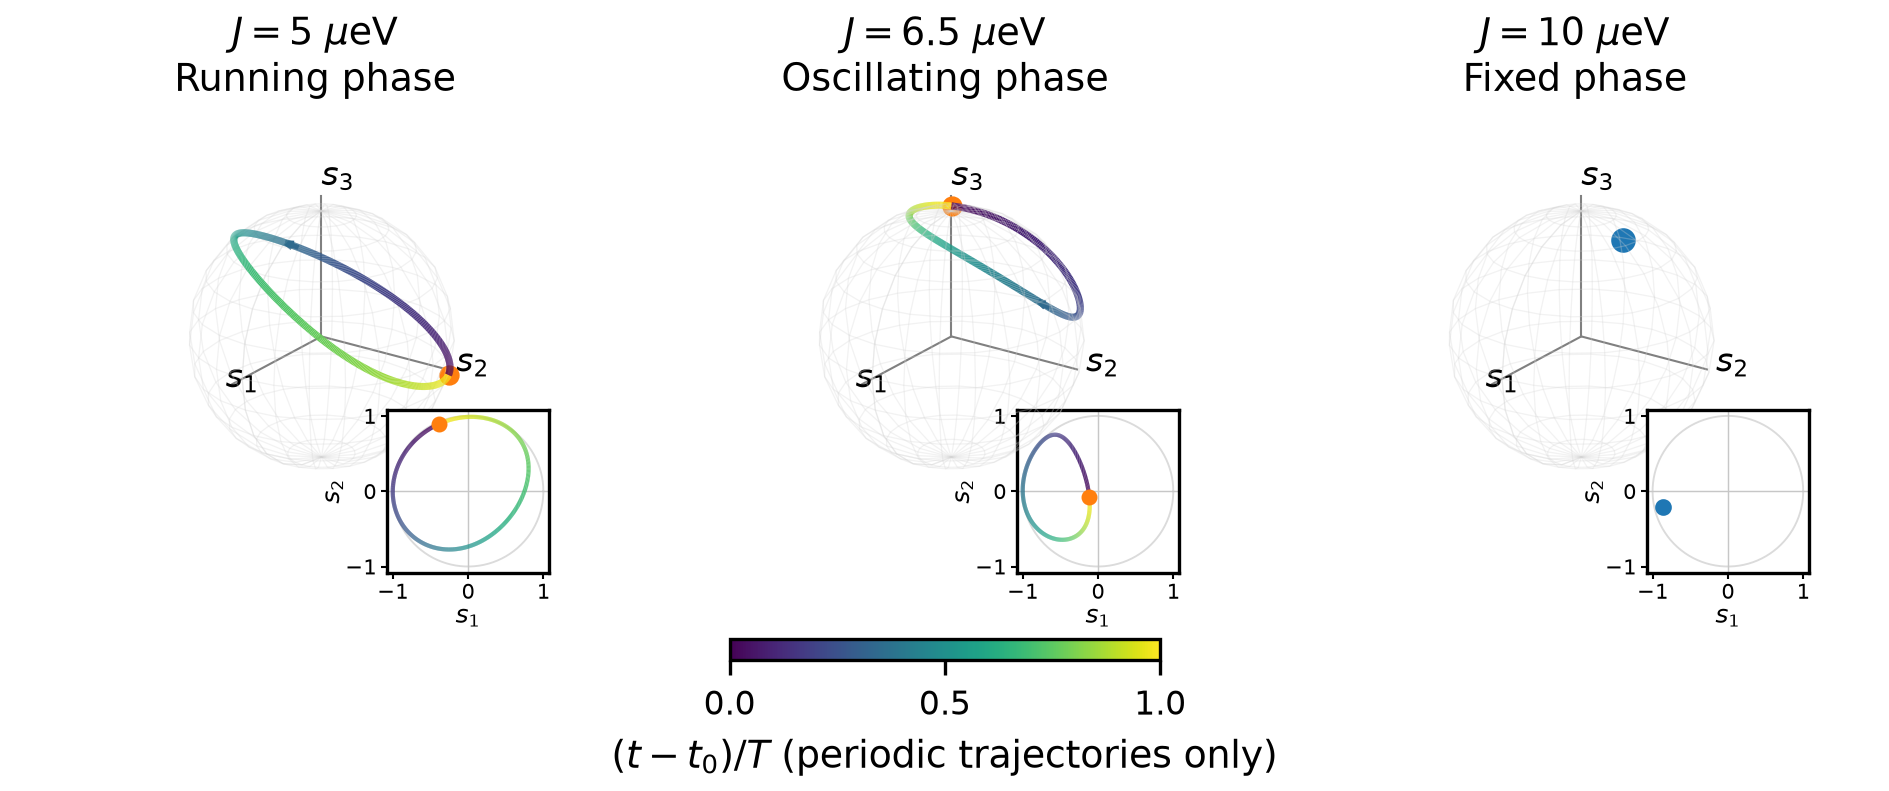
\includegraphics[width=0.96\textwidth]{../results/figures/report3/N10_homogeneous_Poincare.png}
\caption{Poincaré-sphere trajectories for the homogeneous states in Figs.~\ref{fig:4}--\ref{fig:5}, at \(J=5\), 6.5, and 10 \ensuremath{\mu}eV. The oscillatory states show the saved samples spanning approximately one cycle, with measured periods 344.48 and 282.41 ps; the stationary state is a point. Sampling intervals are given in Table~\ref{tab:sampling}. Color denotes \((t-t_0)/T\), arrows indicate motion, and a marker identifies each start. Instantaneous fields give \(|\mathbf s|=1\), without averaging.}
\label{fig:15}
\end{figure}

\subsection{Polarization dynamics at the center of the 2D spot}

Figure 16 uses only \(\mathbf s(0,0,t)\) from the 40, 65, and 100 \ensuremath{\mu}eV calculations of Fig.~\ref{fig:12}. All three trajectories start at \(t_0=2600\) ps. Each oscillatory state is shown over one local period \(T_c\); the stationary state is a point. Sphere axes and viewing angles are identical.

The scan, time traces, and sphere plots thus connect coupling strength, phase classification, and polarization geometry. No additional dynamical approximation is introduced by the sphere representation.


\begin{figure}[H]
\centering
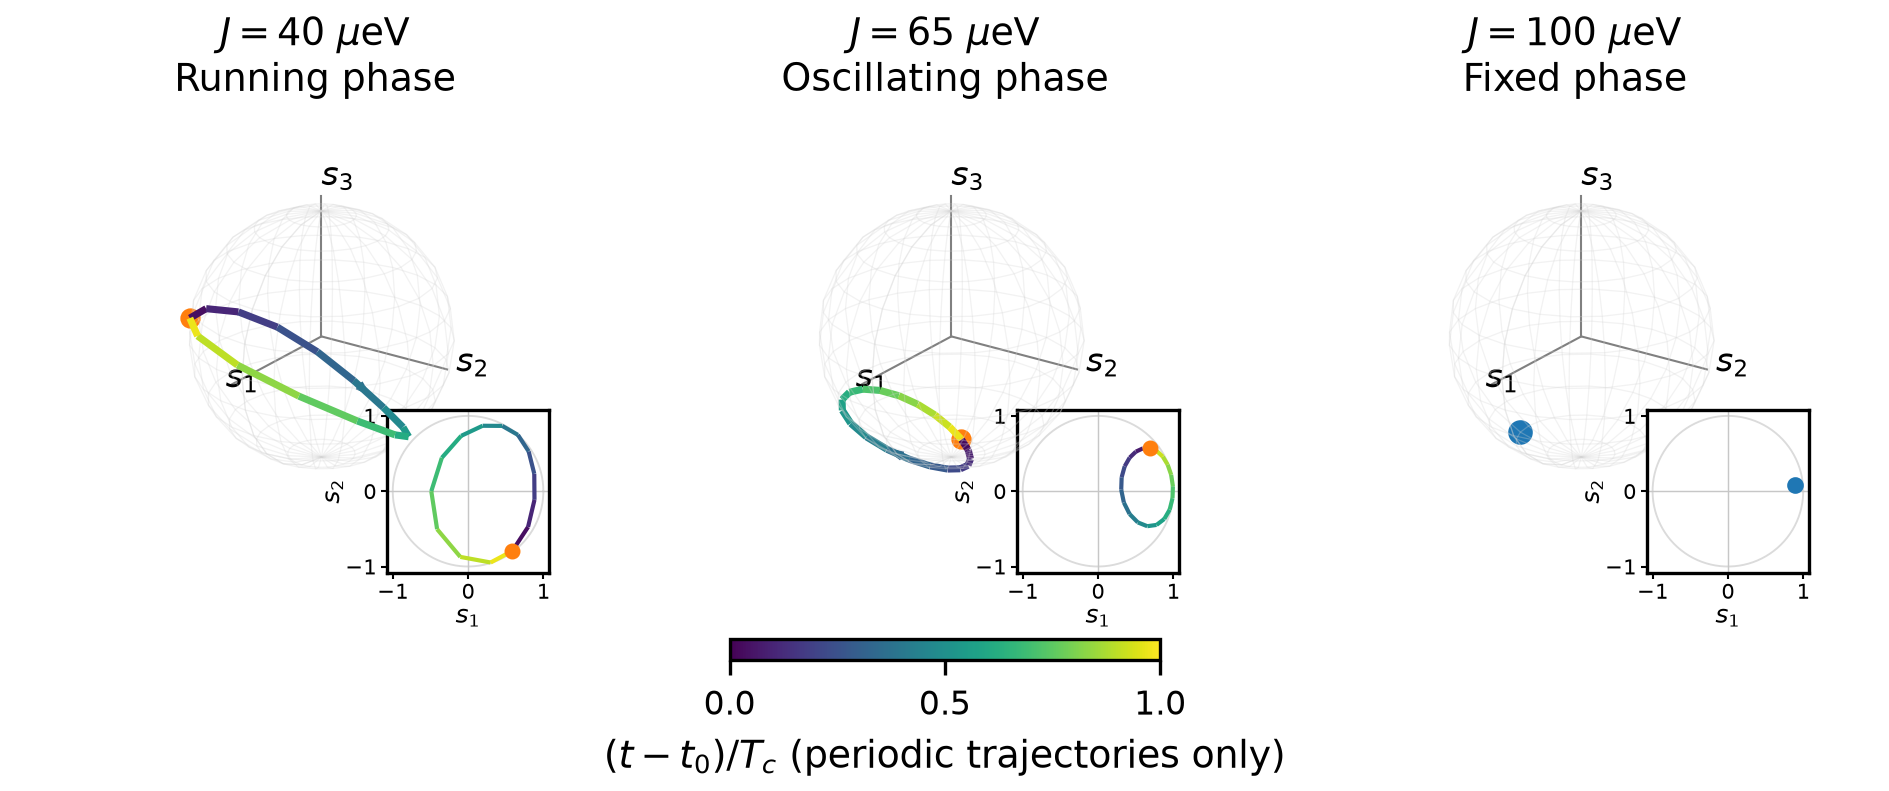
\includegraphics[width=0.96\textwidth]{../results/figures/report3/N11_spot_Poincare.png}
\caption{Local Poincaré-sphere trajectories at the Gaussian-spot center for \(J=40\), 65, and 100 \ensuremath{\mu}eV, using the same \(256^2\) calculations as Fig.~\ref{fig:12}. All cases start at \(t_0=2600\) ps. The running and bounded-phase states show one local period, \(T_c\approx34.6402\) and \(25.0861\) ps, respectively; the fixed state is a point. Color denotes \((t-t_0)/T_c\), with arrows and start markers. No spatial averaging is applied; all panels use the same scale and view. Cycle endpoints are interpolated in unnormalized Stokes components and then divided by \(S_0\), without an artificial closing segment or forced unit normalization. Sampling details are listed in Table~\ref{tab:sampling}.}
\label{fig:16}
\end{figure}


\clearpage
\begingroup\footnotesize\setlength{\tabcolsep}{5pt}\renewcommand{\arraystretch}{1.2}
\begin{longtable}{@{}p{0.24\textwidth}p{0.72\textwidth}@{}}
\caption{Snapshot times and analysis settings. Radii are measured from the pump center; times are measured from the simulation start. Populations are integrated over the full computational domain. Rounded values are reported at the times of the displayed snapshots.}\label{tab:sampling}\\
\toprule
Figure & Sampling and analysis settings\\
\midrule
3(a,b): spot & \(t=3000\) ps; \(N_+=116.277\), \(N_-=93.7473\), \(Z=0.107274\).\\
3(c,d): ring & \(t=6000\) ps; \(N_+=516.265\), \(N_-=241.631\), \(Z=0.362365\).\\
7 & Spot snapshot at \(t=3000\) ps.\\
8 & Ring snapshot at \(t=6000\) ps.\\
9 & Analysis annulus \(5\le r\le15\;\mu\mathrm m\); all four runs use \(2600\le t\le3000\) ps.\\
10 & Radial interval \(5\le r\le7.5\;\mu\mathrm m\). No coherent coupling: 6000 ps; TE--TM only: 6000 ps; \(J\) only: 3600 ps; \(J+\mathrm{TE\text{–}TM}\): 3600 ps.\\
12 & All central traces start at \(t_0=2600\) ps. Each oscillatory example spans three confirmed local periods; the fixed-state example uses a comparable duration.\\
13 & Spot Stokes maps at \(t=2600\) ps, \(J=40\) \ensuremath{\mu}eV: the initial snapshot of the corresponding central trajectory.\\
14 & Ring Stokes maps at \(t=3600\) ps, \(J=10\) \ensuremath{\mu}eV.\\
15 & Homogeneous samples: 17000--17344 ps at 5 \ensuremath{\mu}eV and 17000--17282 ps at 6.5 \ensuremath{\mu}eV, sampled every 0.5 ps; the 10 \ensuremath{\mu}eV fixed-state point is taken at 18000 ps.\\
16 & One central cycle: 2600--2634.6402 ps at 40 \ensuremath{\mu}eV and 2600--2625.0861 ps at 65 \ensuremath{\mu}eV. The 100 \ensuremath{\mu}eV fixed state is represented by its point at 2600 ps.\\
\bottomrule
\end{longtable}
\endgroup

\section*{Conclusions}

Matching the active--inactive cascade to the earlier scalar model preserves its stationary solutions and homogeneous threshold while changing transients. At \(P_A=1.5P_{\rm th}\), the half-density arrival is delayed from 159.1 to 188.0 ps, and decay after pump removal is slower.

Reservoir spin relaxation reduces the pump-induced imbalance; the homogeneous steady densities agree with the analytical solution. Constant coherent coupling produces three distinct regimes: a running relative phase, bounded phase oscillations, and a fixed phase. Cessation of phase accumulation and disappearance of density oscillations occur at different couplings.

TE--TM coupling creates spatial circular-polarization structure under equal pumping. For the spot, the second angular harmonic grows approximately linearly across the sampled coupling range. In the annular comparison, adding constant coupling changes the displayed angular profile from four maxima to two. The three dynamical regimes also appear in the 2D spot, illustrated at 40, 65, and 100 \ensuremath{\mu}eV. Stokes maps and central sphere trajectories connect these regimes to the polarization state.

The numerical evidence has different scope: the main spatial comparisons use \(512^2\), with independent controls for the combined-coupling references, whereas the selected high-\(J\) examples use \(256^2\). Their transition boundaries are not yet grid-converged. The equal-pump TE--TM ring still shows slow polarization evolution at 6000 ps. Finally, additional coefficients are literature-scale model choices rather than a common experimental calibration; the results establish behavior of this specified model and preparation.

\clearpage
\appendix
\section{Parameters and their relation to the previous reports}

\subsection{Parameters retained from the condensation model}

The base coefficients are retained from the previous report, which used the parametrization of Alyatkin et al. \cite{ref1}. In particular, \(R\) is a model parameter and \(g_R=2g_C\) is an assumption of that model. Retaining these values makes the comparison consistent; it does not imply that every coefficient was independently measured for the structure considered here.

\begingroup\small\setlength{\tabcolsep}{5pt}\renewcommand{\arraystretch}{1.2}
\begin{longtable}{@{}p{0.24\textwidth}p{0.72\textwidth}@{}}
\toprule
Quantity & Value\\
\midrule
\(\hbar\) & 0.658212 meV ps\\
\(m/m_e\) & \(5.63\times10^{-5}\)\\
\(K=\hbar^2/(2m)\) & 0.676729 meV \ensuremath{\mu}m\textsuperscript{2}\\
\(g_C=\alpha_1\) & 0.0024 meV \ensuremath{\mu}m\textsuperscript{2}\\
\(g_R=g_A\) & 0.0048 meV \ensuremath{\mu}m\textsuperscript{2}\\
\(R\) & 0.021 \ensuremath{\mu}m\textsuperscript{2} ps\textsuperscript{-}\textsuperscript{1}\\
\(\gamma_C\) & 0.182 ps\textsuperscript{-}\textsuperscript{1}\\
\(\gamma_R=\gamma_A\) & 0.050 ps\textsuperscript{-}\textsuperscript{1}\\
\(\eta\) & 9.8 ps\\
\bottomrule
\end{longtable}
\endgroup

All densities are expressed in \ensuremath{\mu}m\textsuperscript{-}\textsuperscript{2} and pump rates in \ensuremath{\mu}m\textsuperscript{-}\textsuperscript{2} ps\textsuperscript{-}\textsuperscript{1}. These are lower-polariton parameters. Neither the polariton mass nor the loss rate is re-extracted from the transfer-matrix model of the first report.

\subsection{Inactive reservoir}

The matching condition \(g_I/W=g_R\eta\) fixes the ratio of two new coefficients, not their individual values. The main parameter set additionally assumes \(g_I=g_R\), giving \(W=1/\eta=0.102041\;\mathrm{ps}^{-1}\).

The inactive-reservoir loss rate is \(\gamma_I=1/550\;\mathrm{ps}^{-1}\), following the scale in Ref. \cite{ref2}. Its other parameters are not adopted as a complete set: \(\gamma_A\) is retained from the condensation report, and \(W\) is fixed by matching. The resulting values are

\[
g_I=0.0048\;\mathrm{meV}\,\mu\mathrm m^2,\qquad
\tau_I=9.62844\;\mathrm{ps},\qquad P_{\rm in}=1.01782P_A.
\]

The 550 ps time describes loss without transfer to the active reservoir. The response of the cascade is governed by the sum \(\gamma_I+W\), hence the much shorter \(\tau_I\).

\subsection{Spin-dependent coefficients and the scalar limit}

We retain \(\alpha_1=g_C\) and choose \(\alpha_2=-0.1\alpha_1=-0.00024\;\mathrm{meV}\,\mu\mathrm m^2\), using the model ratio in Ref. \cite{ref4}. The reservoir rates are \(\Gamma_{s,A}=\Gamma_{s,I}=0.1\;\mathrm{ps}^{-1}\), following the scale used in Ref. \cite{ref3}. These are parameters of a phenomenological extension, not measurements of the present structure.

For a term \(\Gamma_s(n_{-\sigma}-n_\sigma)\), spin exchange alone makes the population difference decay at \(2\Gamma_s\), corresponding to 5 ps for this choice. This factor must be included when comparing relaxation-time conventions.

The spinor model reduces exactly to the scalar two-reservoir model when \(J=\beta=\Gamma_{s,A}=\Gamma_{s,I}=0\), the minus pump is zero, and all minus fields and densities initially vanish. The zero minus component is then preserved. This limit differs from symmetric pumping of two occupied components. The stationary matching of Eq. (3) applies to the scalar models and does not equate their arbitrary transients.

\subsection{Constant coherent coupling}

The reference \(J=0.010\) meV corresponds to a linear polarization splitting \(2J=20\;\mu\mathrm{eV}\) for equal diagonal energies. Splittings of approximately 15--20 \ensuremath{\mu}eV were reported by Paraïso et al. \cite{ref5} for another microcavity. This provides a reference energy scale, not a calibration of the present sample.

The homogeneous and spatial scans vary \(J\) independently of the other coefficients. The larger values explored in the spatial scan are a model study; their entire range is not justified as a measured splitting by the 15--20 \ensuremath{\mu}eV reference.

\subsection{TE--TM coefficient}

The new coefficient is taken from the lower-polariton model of Cilibrizzi et al. \cite{ref6}:

\[
\beta_{\rm ref}=\frac{\Delta_{LT}}{k_{LT}^2}
=11.9\;\mu\mathrm{eV}\,\mu\mathrm m^2
=0.0119\;\mathrm{meV}\,\mu\mathrm m^2.
\]

In that convention, \(\Delta_{LT}\) is half the TE--TM splitting at \(k_{LT}\); no additional division by two is needed. The coefficient already belongs to a polariton equation, so no extra photon-fraction factor is applied. It is adopted as a literature scale, not as a fit to our cavity.

The retained curvature satisfies \(K>|\beta|\) throughout the chosen range. For \(\beta_{\rm ref}\), the splitting at \(k=1\;\mu\mathrm m^{-1}\) is 23.8 \ensuremath{\mu}eV. The sensitivity calculations use \(0\), \(0.5\beta_{\rm ref}\), \(\beta_{\rm ref}\), and \(2\beta_{\rm ref}\).

For calibration to a particular structure, the lower-polariton TE and TM dispersions would have to be calculated for that same structure and detuning, then fitted at small \(k\) by their quadratic difference. The present extension does not perform that additional transfer-matrix calculation. In particular, the 2×2 photon--exciton matrix in the dispersion report and the 2×2 circular-polarization operator here act on different degrees of freedom.

\section{Numerical method and validation}

\subsection{Homogeneous integration and initial states}

In the homogeneous calculations, spatial derivatives are omitted, but two-dimensional density units are retained. The fields and reservoirs are integrated jointly with DOP853, with relative and absolute tolerances \(2\times10^{-11}\) and \(2\times10^{-13}\). The retained 0D series starts from

\[
\psi_\pm(0)=\sqrt{5\times10^{-5}}\,e^{\pm0.1i},\qquad
n_{A,\pm}(0)=n_{I,\pm}(0)=0.
\]

Steady states at \(J=0\) are checked against Eq. (7). Periodic candidates require recurring densities and polarization, stable periods, and persistent amplitudes on extended windows. Slow cases are integrated longer. Figures 4--6 retain the same original 0D series and initial conditions.

The spatial spot starts from \(\psi_\pm(\mathbf r,0)=\sqrt{10^{-4}f(r)/2}\), with zero relative phase and empty reservoirs. Annular runs multiply both components by the same smooth real perturbation of amplitude \(10^{-3}\), evaluated continuously on each grid. This imposes no circulation and replaces the earlier 24-plane-wave seed.

\subsection{Grid and Fourier step}

The main spatial comparisons use a periodic \(256\times256\;\mu\mathrm m\) domain, a \(512\times512\) grid, and \(\Delta t=0.025\) ps. Two complex condensate fields and four real reservoir densities are evolved in double precision; \(n_\pm\) are evaluated from the fields rather than integrated as independent variables.

For a square periodic domain, \(k_x=2\pi m_x/L\) and \(k_y=2\pi m_y/L\), where \(m_x,m_y\) are the signed discrete Fourier indices. With \(\widetilde\psi(\mathbf k)=\int\psi(\mathbf r)e^{-i\mathbf k\cdot\mathbf r}\,d^2r\), spatial differentiation becomes multiplication by \(ik_x\) or \(ik_y\). The kinetic and TE--TM operator is

\[
H_F=Kk^2\mathbb I+B(\mathbf k),\qquad
B(\mathbf k)=\beta\begin{pmatrix}
0&(k_x-ik_y)^2\\
(k_x+ik_y)^2&0
\end{pmatrix}.
\tag{24}\label{eq:24}
\]

Since \(B^2=\beta^2 k^4\mathbb I\), the exact Fourier propagator over \(\tau\) is

\[
U_F(\tau)=e^{-iKk^2\tau/\hbar}
\left[\cos u\,\mathbb I-i\frac{\tau}{\hbar}\operatorname{sinc}(u)B\right],
\qquad u=\frac{\beta k^2\tau}{\hbar},\qquad
\operatorname{sinc}(u)=\frac{\sin u}{u}.
\tag{25}\label{eq:25}
\]

The continuous value \(\operatorname{sinc}(0)=1\) is used at zero argument. For \(\beta=0\), this reduces to the previous scalar kinetic multiplier applied separately to each component.

Each time step consists of a Fourier half-step, a joint local fourth-order Runge--Kutta step, and a second Fourier half-step. The local field equations are

\[
\partial_t\psi_\sigma=
\left[\frac{Rn_{A,\sigma}-\gamma_C}{2}-\frac{iV_\sigma}{\hbar}\right]\psi_\sigma
+\frac{iJ}{\hbar}\psi_{-\sigma},
\tag{26}\label{eq:26}
\]

together with the four reservoir equations. All quantities are updated jointly at each Runge--Kutta stage. This real-space operation is not an exact exponential with frozen densities. The combined splitting scheme is second-order accurate in time. The constant coupling \(J\) is included in this local step only, not again in Eq. (24).

The propagator can be checked independently through the \(\beta=0\) limit, preservation of the spinor norm during the isolated Fourier step, and the plane-wave eigenenergies \((K\pm\beta)k^2\). For an initially pure + plane wave evolved by this operator alone, the minus population fraction is \(\sin^2(\beta k^2t/\hbar)\).

\subsection{Dynamical classification and spatial controls}

Population stationarity is checked separately for each component and reservoir. The criteria include less than 0.5\% relative variation of each population and less than 1\% changes in the corresponding density maps over consecutive late windows. A stationary polarization additionally requires stable Stokes maps. Constant total population alone is insufficient.

For periodic candidates, each of two consecutive analysis windows contains at least five periods and is at least 200 ps long. The period, mean values, amplitudes, and map recurrence must agree within the stated tolerances. The comparison includes both condensate densities, all four reservoirs, and the polarization maps. Nearly vanishing spatial integrals of linear Stokes components are not used to reject a cycle whose local maps remain periodic. If the available history or sampling does not resolve the test, the classification remains unresolved.

The independent half-step and \(768^2\) tests of the \(J=10\;\mu\mathrm{eV}\), \(\beta=\beta_{\rm ref}\) references are quantified in Section 4.3. Comparisons use common spatial coordinates; the periodic spot allows one recorded common cycle shift. Its full-map recurrence period is approximately 53.68 ps. The ring is stationary. These tests do not constitute a completed \(1024^2\) calculation or a strict error bound.

The larger-domain test supports the combined-coupling reference within the adopted tolerances. It does not validate every scan point. The \(256^2\) scan has selected grid, step, and domain controls; its high-\(J\) central examples remain less thoroughly checked than the \(512^2\) references. Local-cycle periods reported in Section 4.4 are not substituted for full-map recurrence tests.

Angular observables use a common spatial quadrature. This separates changes in the propagated fields from changes caused by discretizing the analysis region. Polarization maps are masked where \(S_0<10^{-3}\max S_0\), using the maximum over the full domain. Relative-phase analysis requires a separate check that neither component becomes too weak; a well-defined total density alone does not guarantee a reliable relative phase.

\clearpage\begin{thebibliography}{6}

\bibitem{ref1} S. Alyatkin et al. \emph{Antiferromagnetic Ising model in a triangular vortex lattice of quantum fluids of light.} Science Advances \textbf{10}, eadj1589 (2024). \url{https://doi.org/10.1126/sciadv.adj1589}

\bibitem{ref2} I. Gnusov et al. \emph{Quantum vortex formation in the ``rotating bucket'' experiment with polariton condensates.} Science Advances \textbf{9}, eadd1299 (2023). \url{https://doi.org/10.1126/sciadv.add1299}

\bibitem{ref3} I. Gnusov et al. \emph{Optical orientation, polarization pinning, and depolarization dynamics in optically confined polariton condensates.} Physical Review B \textbf{102}, 125419 (2020). \url{https://doi.org/10.1103/PhysRevB.102.125419}

\bibitem{ref4} A. Askitopoulos et al. \emph{Nonresonant optical control of a spinor polariton condensate.} Physical Review B \textbf{93}, 205307 (2016). \url{https://doi.org/10.1103/PhysRevB.93.205307}

\bibitem{ref5} T. K. Paraïso et al. \emph{Multistability of a coherent spin ensemble in a semiconductor microcavity.} Nature Materials \textbf{9}, 655--660 (2010). \url{https://doi.org/10.1038/nmat2787}

\bibitem{ref6} P. Cilibrizzi et al. \emph{Half-skyrmion spin textures in polariton microcavities.} Physical Review B \textbf{94}, 045315 (2016). \url{https://doi.org/10.1103/PhysRevB.94.045315} ; author manuscript: \url{https://arxiv.org/abs/1602.04711}


\end{thebibliography}
\end{document}
